\documentclass[a4paper]{article}
\usepackage[utf8]{inputenc}
\usepackage{fullpage}
\usepackage{enumitem}
\usepackage{todonotes}
\usepackage{graphicx}
\usepackage{array}
\usepackage{mdwlist}
\usepackage{floatrow}
\usepackage{hyperref}
\usepackage{listings}
\usepackage{alloy}
\usepackage{color}

\graphicspath{ {img/} }

\let\stdsection\section
\renewcommand\section{\newpage\stdsection}

\title{{\Huge myTaxiService} \\ Requirements Analysis and Specifications Document}
\author{Jacopo Strada \and Luca Riva}
\date{November 6, 2015}

\begin{document}

\maketitle

\newpage

\tableofcontents

\listoffigures 

\listoftables

\setlength{\parindent}{0em}
\setlength{\parskip}{1em}

\section{Introduction}
\subsection{Purpose}
This document is meant to describe a software solution for the \emph{myTaxiService} problem. The document includes a description of the problem, functional and non-functional requirements and it is addressed to the IT department of the city administration.

\subsection{Scope}
The \emph{myTaxiService} software focuses on helping the clients benefit from the service and ensures a fair management of taxi queues.

The software will:

\begin{itemize}
\item give the possibility to request a taxi either through a web application or a mobile app.
\item compute the distribution of taxis in the various zones based on the GPS information it receives from each taxi.
\item offer programmatic interfaces to enable the development of additional services.
\item allow to book a taxi by specifying the origin and the destination of the ride.
\end{itemize}

\subsubsection{Goals}

\begin{enumerate}[label=\bfseries G\arabic*:]
\item Allow clients to register an account in the system
\item Allow taxi drivers to register an account in the system
\item Allow clients to log in the mobile application or in the website
\item Allow taxi drivers to log in the mobile application
\item Allow clients to request a taxi
\item Inform the passenger about the code of the incoming taxi
\item Inform the passenger about the waiting time
\item Inform the passenger about a possible call rejection
\item Retrieve the position of each taxi from their mobile application using GPS
\item Allow taxi drivers to set their state as \emph{available} or \emph{unavailable}
\item Notify the taxi drivers about a client's request
\item Allow taxi drivers to accept or decline a certain client's request
\item Guarantee a fair management of taxi queues
\item Allow a user to reserve a taxi by specifying the origin and the destination of the ride at least two hours before
\item Allow a driver to accept a client reservation
\item Confirm the reservation to the user
\item Supply APIs for further implementation of additional services in the future
\end{enumerate}

\subsection{Glossary}
\subsubsection{Definitions}
\begin{description}
\item[Client / Passenger / User :] Is a person who signed up for this service and their interest is to call a taxi or reserve  a ride.
\item[Taxi Driver :] Is a person who drives a taxi and would like to be called or reserved for a ride through this service.
\end{description}

\subsubsection{Acronyms}
\begin{description}
\item[API:] Application Programming Interface
\item[BPMN:] Business Process Model and Notation
\item[CPU:] Central Processing Unit
\item[GPS:] Global Positioning System
\item[HTTPS:] Hyper Text Transfer Protocol over Secure Socket Layer
\item[IEEE:] Institute of Electrical and Electronics Engineers
\item[IT:] Information Technology
\item[RAM:] Random Access Memory
\item[SSD:] Solid State Drive 
\item[UML:] Unified Modeling Language
\end{description}

\subsubsection{Abbreviations}
\begin{description}
\item[A\emph{n}:] Assumption number \emph{n}
\item[D\emph{n}:] Domain Property number \emph{n}
\item[G\emph{n}:] Goal number \emph{n}
\item[R\emph{n}:] Requirement number \emph{n}
\end{description}

\subsection{References}
\begin{itemize}
\item "myTaxiDriver" Specification Document
\item IEEE Std 830-1998 IEEE Recommended Practice for Software Requirements Specifications
\end{itemize}

\subsection{Document Overview}
\vbox{
\begin{itemize}
\item In section 2 many factors influencing the system and its requirements are explained without emphasizing specific requirements, but focusing on what lays behind the process of defining these requirements and making them easily understandable.
\item In section 3 all the requirements mentioned before are carefully described: inputs and outputs of the system are accounted as well as the processes performed by the system from the reception of a given input to the resulting output. In order to make the requirements and the processes as clear as possible this section includes many models that may help the reader figuring out every important detail.
\item In the appendix of the document it is possible to find an Alloy model of the system's structure with various demonstrations of how the specified requirements guarantee the desired behaviours and properties of the software.
\end{itemize}
}

\section{Overall Description}
\subsection{Product Perspective}
The software will consist in three different user interfaces: two different apps for the clients and the taxi drivers and one web application. 

In order to make this working there will be a web server containing the application logic and a DBMS that stores all the data (such as users' credentials, taxi's positions, taxi's availability \ldots).
Mobile applications, web application and the server communicate through the Internet.

The system will also provide programmatic interfaces for other new services. At the moment the city has not any similar system, so the application will be completely independent.
\subsubsection{User interfaces}

\begin{itemize}
\item Taxi Driver
    \begin{itemize}
    \item Smartphone App on
        \begin{itemize*}
        \item Android
        \item iOS
        \item Windows Phone
        \end{itemize*}
    \item Web Browser (any operating system)
    \end{itemize}
\item Clients
    \begin{itemize}
    \item Smartphone App on
        \begin{itemize*}
        \item Android
        \item iOS
        \item Windows Phone
        \end{itemize*}
    \item Web Browser (any operating system)
    \end{itemize}
\end{itemize}

\subsubsection{Hardware Interface}
Client Side:
\begin{itemize}
\item Smartphone and Tablet
    \begin{itemize}
    \item Android
        \begin{itemize*}
        \item CPU: DualCore 1Ghz
        \item RAM: 700Mb
        \item GPS
        \end{itemize*}
    \item iOS
        \begin{itemize*}
        \item iPhone 4 or greater
        \item iPad 2 or greater
        \end{itemize*}
    \item Windows Phone
        \begin{itemize*}
        \item CPU: DualCore 1Ghz
        \item RAM: 512Mb
        \item GPS
        \end{itemize*}
    \end{itemize}
\item \begin{samepage} Web Browser (any operating system)
        \begin{itemize*}
        \item CPU: 1Ghz
        \item RAM: 1Gb
        \item GPS
        \end{itemize*} \end{samepage}
\end{itemize}

Server Side:
\begin{itemize}
\item 4 Cores, 2.8-3.0 GHz each (2.8 GHz minimum speed)
\item 4 GB RAM per core
\item SSD, 100 GB
\end{itemize}

\subsubsection{Software Interfaces}
\begin{itemize}
\item Google Maps API V3
\item Taxi drivers' licences database V1
\end{itemize}

\subsubsection{Communications Interfaces}
All the applications will use HTTPS protocol.

\subsection{User characteristics}
This application is conceived for every taxi driver in the city area and for adult clients (18+) with a compatible device which satisfies the specification listed in the previous section. There are no specific levels of education or expertise needed apart from a decent knowledge of English language.

\subsection{Constraints}
\begin{description}
\item[Interfaces to other applications:] Google Maps will be integrated in the system in order to give clear information about a client position and allow the client to modify a wrong position calculated by their smartphone's GPS. Another important feature that this service will offer is the computation of an estimated waiting time for the taxi to reach the client.
\item[Parallel Operations:] The system is studied for a large city with an high usage of taxi service. So parallelism is very important because a lot of taxi calls may income in the same time and a lot of taxi drivers have to been indexed by the system.
\item[Reliability requirements:] In order to keep an high level of service the system must be reliable. Each call must reach a taxi driver and a response has to arrive to the user in a reasonable time (5 min).
\end{description}

\subsection{Domain properties}
\begin{enumerate}[label=\bfseries D\arabic*:]
\item If a client requests a ride they will wait the taxi's arrival
\item If a client makes a reservation for a certain time they will be punctual waiting for the ride
\item If a driver accepts a reservation or a request they will actually try to reach the client location

\end{enumerate}

\subsection{Assumptions}
\begin{enumerate}[label=\bfseries A\arabic*:]
\item Possibility to gain access to the taxi driver's licences database of the city
\item A client is able to make only one taxi request at once
\item A client is not able to make two overlapped reservations
\item If a request is rejected by all the taxi drivers in the queue the request will be discarded: it will not iterate the queue for a second time.
\item As soon as the request is discarded the client will be notified and able to make a new call
\item The system will not give the client any information regarding the cost of the ride
\item If a client calls a taxi and the request is accepted the client will not be able to modify or erase the request.
\end{enumerate}

In order to assure an efficient service it is necessary a slight modification to the customer request:

\begin{enumerate}[label=\bfseries A\arabic*:, resume]
\item When a customer reserves a taxi the system allocates the request to all registered driver
\item If a driver accepts the request the system confirms the reservation to the user
\item If no driver confirms the reservation in at most an hour since the request the system deletes the reservation and notifies the client
\item A taxi reservation's origin must be located inside one of the zones of the city
\item A client is able to cancel a reservation at least ten minutes before the ride.
\item The system notifies the driver about the ride they accepted ten minutes before the hour of the appointment with the client
\end{enumerate}

Assumptions A8, A9, A10, A13 were made in order to avoid the risk of having an empty queue or no driver who would accept the reservation only ten minutes before the fixed hour of the ride.

\subsection{Apportioning of requirements}
\begin{description}
\item[Reporting:] A client may report the lack of service of a driver so that the city's government would be able to take action against the said driver. At the same time a driver may be able to report a client who misses fixed appointments, thus after few reclaims the client's account could be suspended or deactivated. 
\item[Payments:] It would be interesting to give the client the possibility to pay the reservation service directly through the system, which could also provide an estimated price for the ride given the origin and the destination.
\item[Taxi sharing:] An user may be ready to share a taxi, so the application could mark their requests in order to allow other clients to participate in the ride if they have a similar starting point and a similar destination. Obviously the advantage wold be the possibility to split the cost of the ride, which should be calculated by the system. The system should also compute the route for the taxi driver.
\end{description}

\section{Specific requirements}

\subsection{Functional Requirements}

\begin{enumerate}[label=\bfseries G\arabic*:]
    \item
        \begin{enumerate}[label=\bfseries R\arabic*:]
        \item Clients must provide a valid e-mail address. It will become the identifier for the account.
        \item Clients must provide their Name, Surname, Date of Birth and a valid Mobile Phone Number
        \item Clients must provide a password with a minimum length of 8 characters
        \item User cannot sign up twice
        \item Visitor can just see log in page and registration form
        \end{enumerate}
    \item
        \begin{enumerate}[label=\bfseries R\arabic*:]
        \item Taxi drivers must provide a valid e-mail address. It will become the identifier for the account.
        \item Taxi drivers must provide their Name, Surname and a valid Mobile Phone Number.
        \item Taxi drivers must provide a password with a minimum length of 8 characters.
        \item Taxi drivers must provide a valid license number which will be verified by the system.
        \item User cannot sign up twice.
        \item Visitor can just see log in page and registration form.
        \end{enumerate}
    \item
        \begin{enumerate}[label=\bfseries R\arabic*:]
        \item Users must be already registered to success login process.
        \item Users must provide their e-mail and password used during the registration process.
        \item If credentials are wrong, the system will reject the login.
        \item The service cannot be used before the login.
        \end{enumerate}
    \item
        \begin{enumerate}[label=\bfseries R\arabic*:]
        \item Taxi drivers must be already registered to success login process.
        \item Taxi drivers must provide their e-mail and password used during the registration process.
        \item If credentials are wrong, the system will reject the login.
        \end{enumerate}
    \item
        \begin{enumerate}[label=\bfseries R\arabic*:]
        \item Users must be already logged in the application.
        \item Users must provide their position.
        \item If the position cannot be retrieved from GPS, the user will have to write the address manually.
        \item If the position retrieved from GPS is not correct or sufficiently precise, the user will have to confirm the detected position or provide the correct one.
        \end{enumerate}
    \item
        \begin{enumerate}[label=\bfseries R\arabic*:]
        \item Users must be already logged in the application.
        \item A taxi driver in the area of the client must have accepted the request
        \end{enumerate}
    \item
        \begin{enumerate}[label=\bfseries R\arabic*:]
        \item Users must be already logged in the application.
        \item A taxi driver in the area of the client must have accepted the request
        \end{enumerate}
    \item
        \begin{enumerate}[label=\bfseries R\arabic*:]
        \item Users must be already logged in the application.
        \item No taxi driver in the area has accepted the client's request
        \end{enumerate}
    \item
        \begin{enumerate}[label=\bfseries R\arabic*:]
        \item Drivers must be already logged in the application.
        \item The application installed on the taxi driver's smartphone must be running in background.
        \item Taxi's current positions must be stored in the central DB with the last update time.
        \end{enumerate}
    \item
        \begin{enumerate}[label=\bfseries R\arabic*:]
        \item Drivers must be already logged in the application.
        \end{enumerate}
    \item
        \begin{enumerate}[label=\bfseries R\arabic*:]
        \item Drivers must be already logged in the application.
        \item Drivers' state must be set as \emph{available}.
        \item Drivers must be in the same zone as the client.
        \item The Smartphone or Tablet must ring or vibrate and display a pop-up for the notification.
        \end{enumerate}
    \item
        \begin{enumerate}[label=\bfseries R\arabic*:]
        \item Drivers must be already logged in the application.
        \item Drivers' state must be set as \emph{available}.
        \item Drivers' state will become \emph{unavailable}.
        \item Drivers must be in the same zone as the client.
        \end{enumerate}
    \item 
        \begin{enumerate}[label=\bfseries R\arabic*:]
        \item System considers the city divided in zones
        \item For each zone exists a queue of taxi drivers
        \item System assigns a driver to a zone basing its decision on their GPS position
        \item System adds a driver to a zone's queue if they are available
        \end{enumerate}
    \item 
        \begin{enumerate}[label=\bfseries R\arabic*:]
        \item System receives taxi requests
        \item System forwards taxi request to the first driver of the queue of client's zone
        \item System sends a confirmation to the client if the driver accepts
        \item System forwards the request to the second driver in the queue if the first one declines
        \item System moves the first driver who has declined to the last position in the queue
        \end{enumerate}
    \item
        \begin{enumerate}[label=\bfseries R\arabic*:]
        \item Clients must be already logged in the application.
        \item Clients must specify a valid origin (see assumption A8).
        \item Clients must make a reservation at least two hours before the ride.
        \end{enumerate}
    \item
        \begin{enumerate}[label=\bfseries R\arabic*:]
        \item System receives a taxi reservation
        \item System forwards request to all the registered drivers
        \item System waits thirty minutes
        \item System stops waiting if a driver accepts the reservation
        \item System sends request's confirmation to the client if a driver has accepted the reservation
        \item System sends a rejection notification to the client if thirty minutes have passed and no driver has accepted the reservation
        \item System notifies the driver who has accepted the reservation ten minutes before the appointment with the client
        \end{enumerate}
    \item
        \begin{enumerate}[label=\bfseries R\arabic*:]
        \item Provide taxi's positions and availability state.
        \end{enumerate}
\end{enumerate}

\subsection{Non Functional Requirements}

\subsubsection{Performance Requirements}

As already stated before, performance is  an important point for this application and so is also necessary to give an idea of the big amount of users who will be serviced by the application.
From a little analysis we have derived that \emph{myTaxiService} has to handle at least 2 Millions of users on line at the same time.

The time of response must be less or equals to 1 second for at least 90\% of transactions.

\subsubsection{Software System Attributes}
\nopagebreak
\vbox{
\begin{description}
\item[Reliability:] The system is a work's provider for Taxi drivers and so it is important not to loose any opportunity. \newline Keeping this in mind a system of acknowledge will be implemented and it will guarantee that all notifications will arrive to their proper destination.
\item[Availability:] This application may become a complete substitute of telephone taxi calls and so it is very important that it will always be available. To do so the system will be hosted on multiple servers in order to be resistant to some faults.]
\item[Security:] The security of the communications is guaranteed by the use of HTTPS with SSL encryption. \newline Attacks are prevented thanks to a structure with more than one level of servers with always a firewall between them.
\end{description}
}

\subsection{External Interfaces}

In this section there is a set of mockups illustrating the most important screens of \emph{myTaxyService}. These mockups are divided into two sections in order to divide the Clients Application from the Taxi Drivers Application.

What is presented is only a first idea of the applications that is useful for a better understanding of the whole system described in next sections.

% Mockups Width
\newlength{\mockupWidth}
\setlength{\mockupWidth}{.3\textwidth}
% Set caption position
\floatsetup[figure]{capposition=beside,capbesideposition={center,right}}

\subsubsection{Clients' User Interfaces}

Here are shown mockups for the Client Application. In the project it is also planned a website for them which is not represented here but it will have the same features proposed for the mobile application.

\begin{figure}[H]
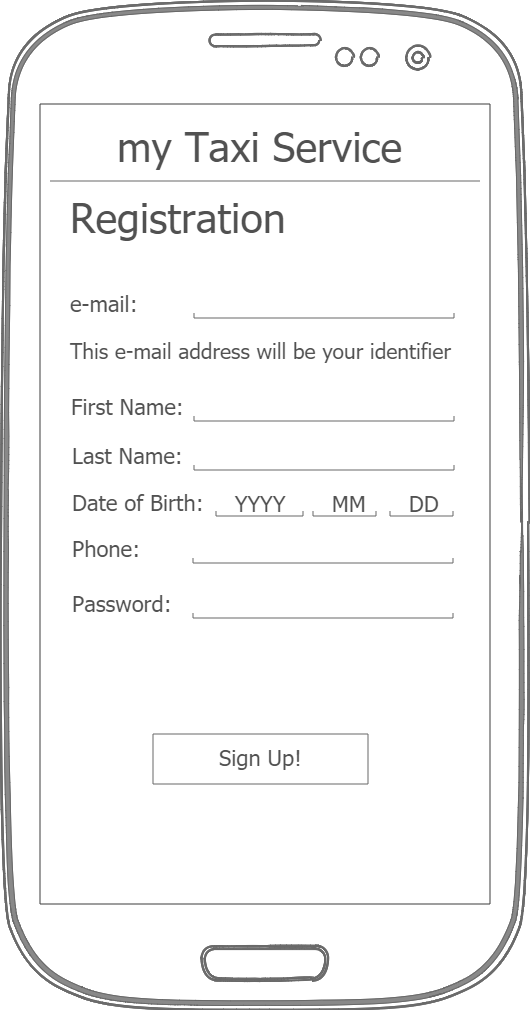
\includegraphics[width=\mockupWidth]{Mockup-ClientsRegistration}
\centering
\caption[Clients Registration Mockup]{Clients Registration Mockup:\newline This is the registration page for a client. All the fields must be filled in correctly in order to register to the service.}
\label{fig:mockupclientregistration}
\end{figure}

\begin{figure}[H]
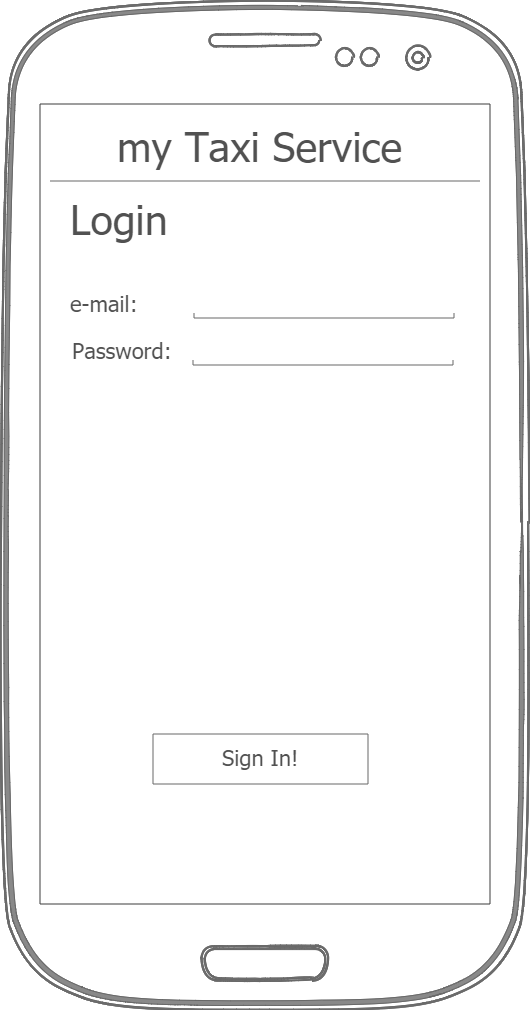
\includegraphics[width=\mockupWidth]{Mockup-ClientsLogin}
\centering
\caption[Clients Login Mockup]{Clients Login Mockup:\newline This page is used to log in and use the application. This is necessary to use every feature of the application.}
\label{fig:mockupclientlogin}
\end{figure}

\begin{figure}[H]
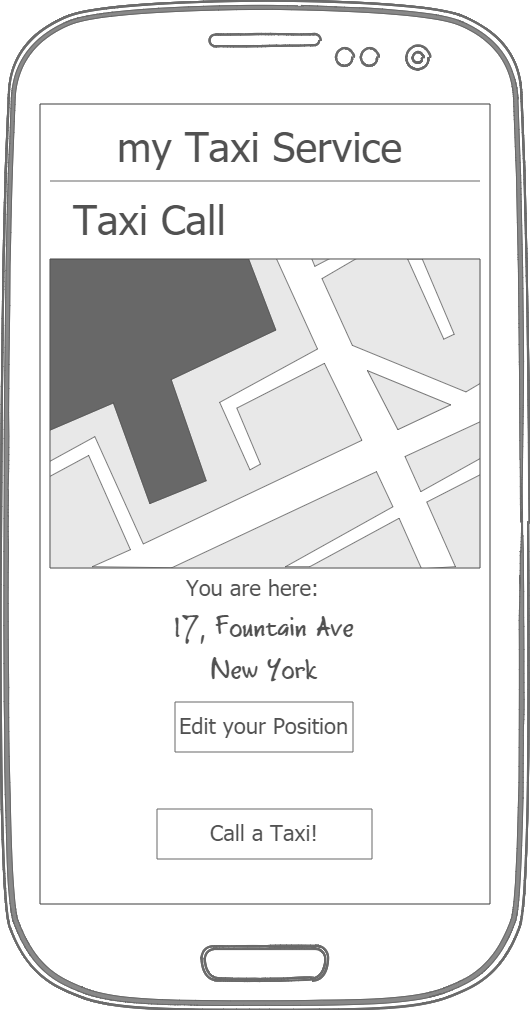
\includegraphics[width=\mockupWidth]{Mockup-ClientsTaxiCall}
\centering
\caption[Clients Taxi Call Mockup]{Clients Taxi Call Mockup: \newline Here is presented the paged used for calling a taxi. The  position retrieved from the GPS (if available) is displayed on the map and written below. The client can use the \emph{Edit your Position} button in order to modify the place in which the taxi will arrive; to do this is provided a page like the which one described in  \autoref{fig:mockupclientfindposition}.}
\label{fig:mockupclienttaxicall}
\end{figure}

\begin{figure}[H]
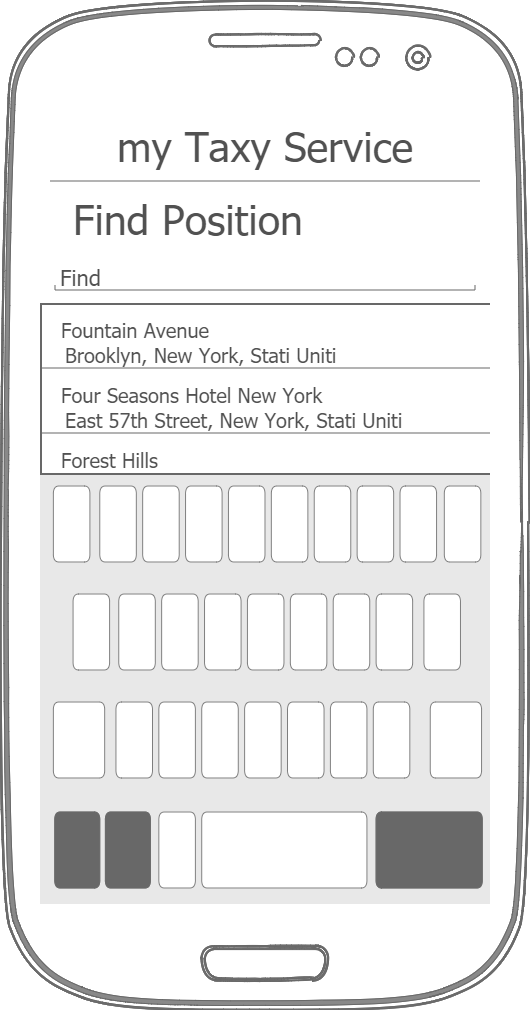
\includegraphics[width=\mockupWidth]{Mockup-ClientsPositionFinder}
\centering
\caption[Find Position Mockup]{Find Position Mockup: \newline This page is used for searching a position. It is possible to type booth street names or places names (such as Hotels, Restaurants \ldots. This utility is called from more than one point of our application: see for example \autoref{fig:mockupclienttaxicall} or  \autoref{fig:mockupclientridereservation}.}
\label{fig:mockupclientfindposition}
\end{figure}

\begin{figure}[H]
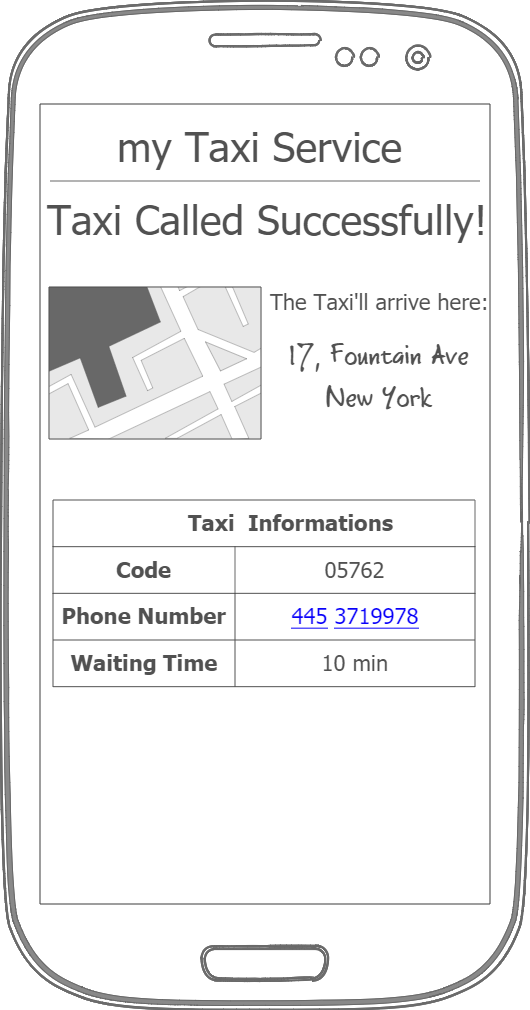
\includegraphics[width=\mockupWidth]{Mockup-ClientsTaxiCallConfirmation}
\centering
\caption[Clients Taxi Call Confirmation Mockup]{Clients Taxi Call Confirmation Mockup: \newline this is what is displayed when a call made by a client was successfully accepted by a taxi driver. This confirmation let the client to know the number of the taxi which will arrive, the taxi driver's phone number and an estimated waiting time.}
\label{fig:mockupclienttaxicallconfirmation}
\end{figure}

\begin{figure}[H]
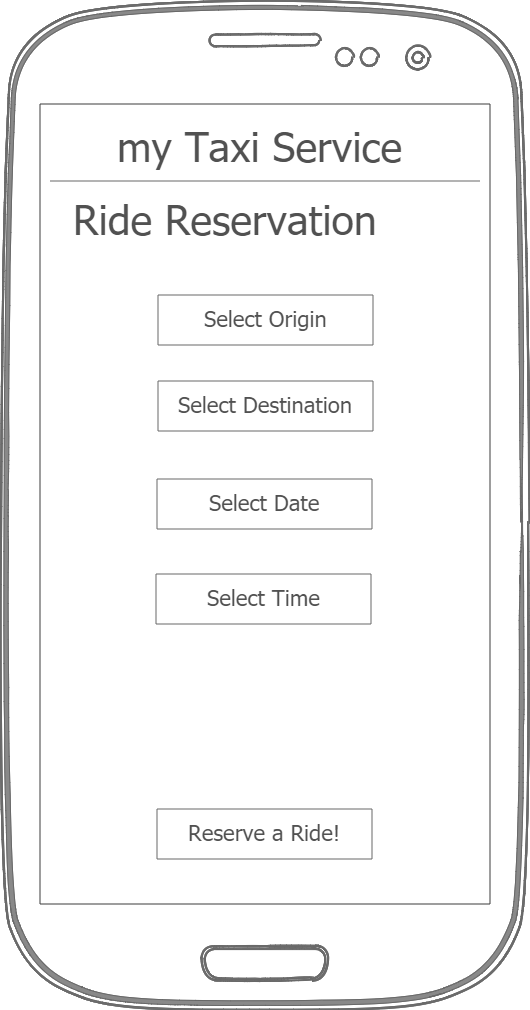
\includegraphics[width=\mockupWidth]{Mockup-ClientsRideReservation}
\centering
\caption[Clients Ride Reservation Mockup]{Clients Ride Reservation Mockup: \newline This page is used to reserve a taxi ride from an origin to a destination specifying a Date and a Time. The two buttons \emph{Select Origin} and \emph{Select Destination} open the utility shown at \autoref{fig:mockupclientfindposition}; the other two open respectively a simple date picker and a simple time picker.}
\label{fig:mockupclientridereservation}
\end{figure}

\subsubsection{Taxi Drivers' User Interfaces}

The following mockups represent the key features of Taxi Drivers' Application.

\begin{figure}[H]
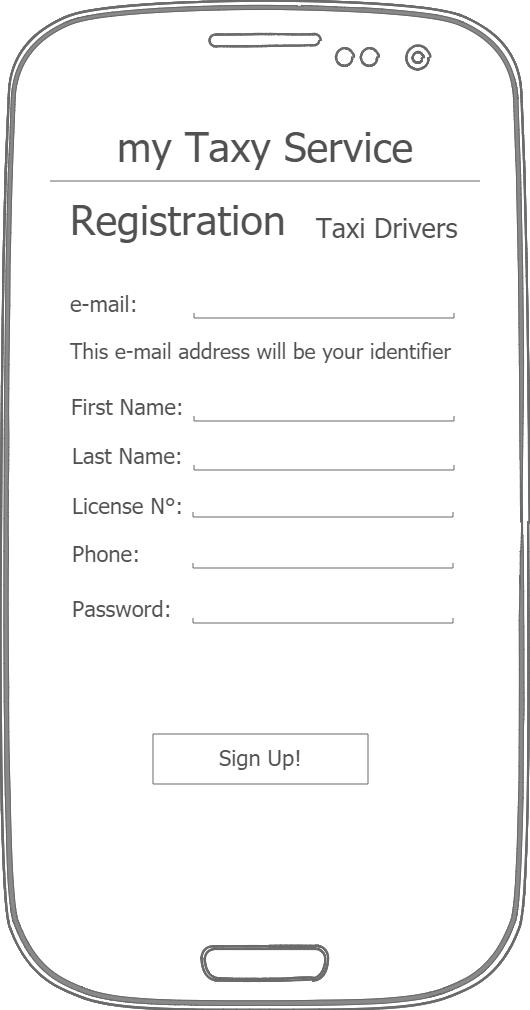
\includegraphics[width=\mockupWidth]{Mockup-TaxiDriversRegistration}
\centering
\caption[Taxi Drivers Registration Mockup]{Taxi Drivers Registration Mockup: \newline This is the registration page for a taxi driver. All the fields must be filled in correctly in order to register to the service.}
\label{fig:mockuptaxidriverregistration}
\end{figure}

\begin{figure}[H]
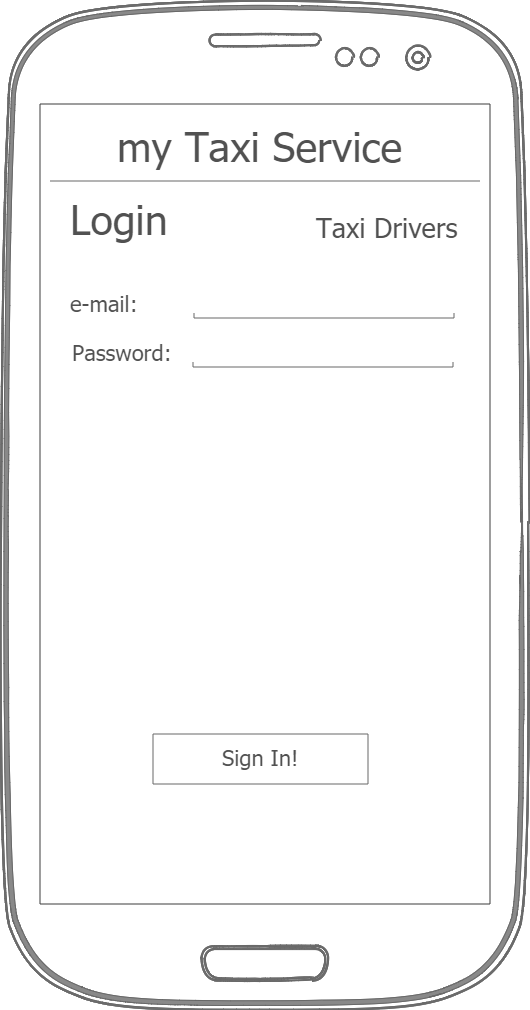
\includegraphics[width=\mockupWidth]{Mockup-TaxiDriversLogin}
\centering
\caption[Taxi Driver Login Mockup]{Taxi Driver Login Mockup:\newline This page is used to log in and use the application. This is necessary to use every feature of the application.}
\label{fig:mockuptaxidriverlogin}
\end{figure}

\begin{figure}[H]
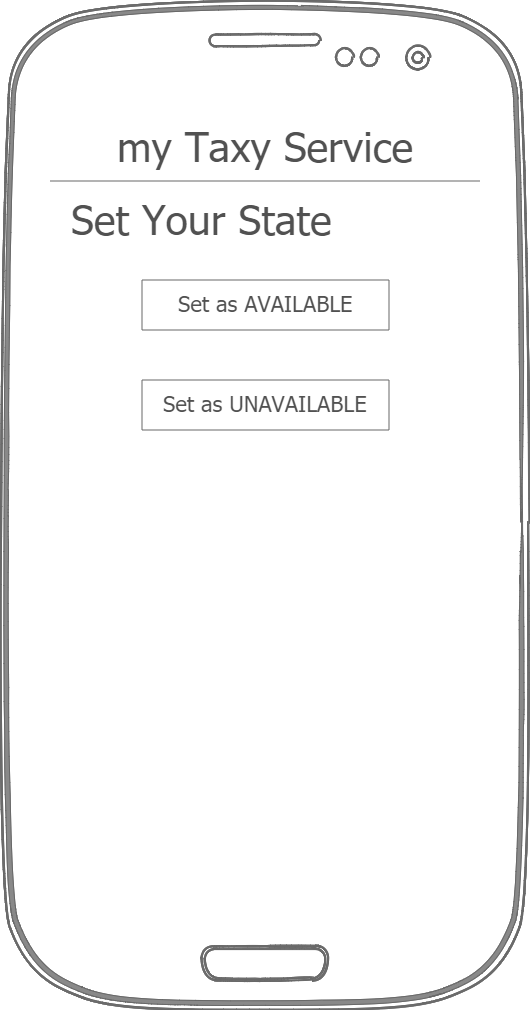
\includegraphics[width=\mockupWidth]{Mockup-TaxiDriversSetStatus}
\centering
\caption[Taxi Drivers Change State Mockup]{Taxi Drivers Change State Mockup: \newline This page is used by taxi drivers in order to set their availability state. To do this they have to click on \emph{Set as AVAILABLE} or \emph{Set as UNAVAILABLE} according to their real state. It is not necessary to use this feature when a taxi driver accepts a call; their state will be set as unavailable automatically.}
\label{fig:mockuptaxidriversetstatus}
\end{figure}

\begin{figure}[H]
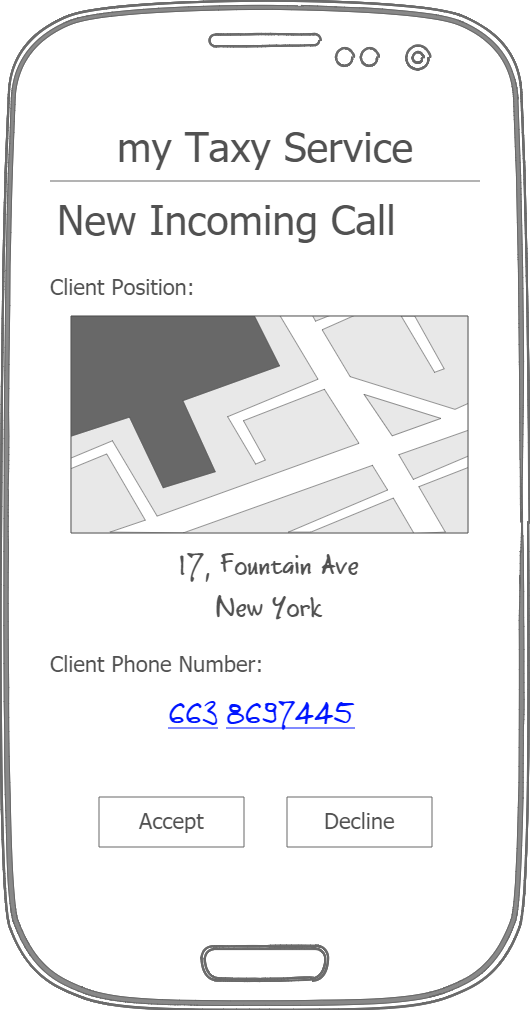
\includegraphics[width=\mockupWidth]{Mockup-TaxiDriversNewIncomingCall}
\centering
\caption[Taxi Drivers Incoming Call Mockup]{Taxi Drivers Incoming Call Mockup: \newline This page is shown when a clients makes a call and the system tries to assign that to a taxi driver. The taxi driver has to click on \emph{Accept} or \emph{Decline} before a timeout expires otherwise the effect is the same of \emph{Decline} and the notification will arrive to the next taxi driver of the queue.}
\label{fig:mockuptaxidriverincomingcall}
\end{figure}

\begin{figure}[H]
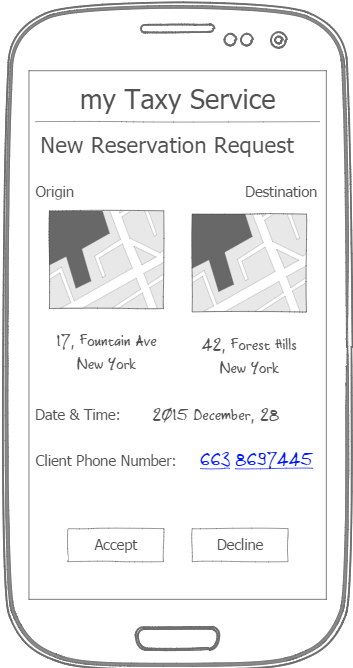
\includegraphics[width=\mockupWidth]{Mockup-TaxiDriversReservationRequest}
\centering
\caption[Taxi Drivers Reservation Request]{Taxi Drivers Reservation Request: \newline This page is shown when a clients makes a reservation request and the system tries to assign that to a taxi driver. The taxi driver has to click on \emph{Accept} or \emph{Decline} before a timeout expires otherwise the effect is the same of \emph{Decline} and the notification will arrive to the next taxi driver of the system.}
\label{fig:mockuptaxidriverireservationrequest}
\end{figure}
\clearpage
\subsection{The World and The Machine}The model by M. Jackson \& P. Zave is able to clearly schematize where the entities involved in the project are ideally located and which are the means of interaction between the world and the system at a first glance.
% Set caption position
\floatsetup[figure]{capposition=bottom}

\begin{figure}[H]
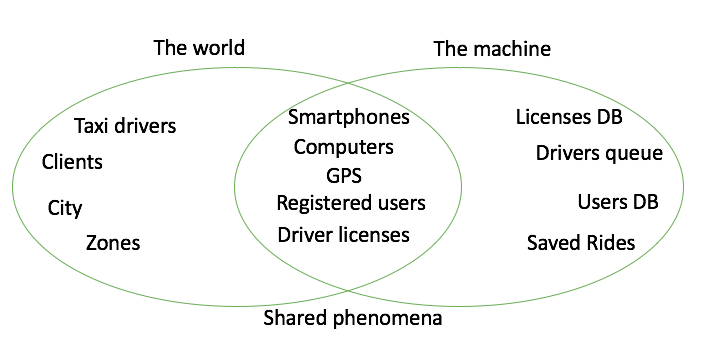
\includegraphics[width=.8\textwidth]{WorldAndMachine}
\centering
\caption{The World and The Machine Representation}
\end{figure}

\subsection{Scenarios}
    \begin{enumerate}[label=\bfseries S\arabic*:]
        \item Goffredo is coming back from work and he notices an advertising billboard of a new app: \emph{myTaxiService}. When he arrives home he fires up his computer and finds out that \emph{myTaxiService} has also a website and he decides to create an account. He clicks on "Register" and fills out the necessary fields. Finally, he clicks "Confirm" and a message appears, communicating that the registration has been successfully performed.
        \item Amerigo has just arrived to the city by plane and he needs a taxi to reach his hotel. Amerigo lives in the city so he already has a registered account for \emph{myTaxiService}. He therefore logs in the application and, after being located by the app, he confirms his position, calculated by the system, and requests a taxi. After a minute Amerigo's phone rings, in fact he has received a notification by "myTaxyService" app. Opening the app he finds the request's confirmation and the expected waiting time
        \item Galla Placidia has been trying the new app \emph{myTaxiService} for a week and, as a taxi driver, she is very happy with it. It's been few minutes since her last ride, so she turns on her phone and opens the app to change her state to "Available" clicking on the proper button: now she is going to be notified if someone in her area asks for a ride.
        \item Arcimboldo is waiting at the taxi parking of the train station for a new request from "myTaxyService". When he hears the notification he opens the app which shows the client's address and position on the map. Arcimboldo quickly accepts the new request, starts the car and leaves the parking lot in order to reach his new client. 
        \item Gianfilippa has been invited to an high school reunion out of town, but she does not have a car and the place is not reachable by the usual public means of transport. Luckily for her a few weeks ago she joined, mostly out of curiosity, \emph{myTaxiService} and thus she has the possibility to book a custom taxi ride. The app asks her to choose an origin and then the destination. After choosing her home and the restaurant, Gianfilippa selects the hour and the date of the reunion and then forwards the reservation. Finally the application reminds her that she will shortly receive a confirmation.
    \end{enumerate}
    
\subsection{UML and BPMN Models}


\subsubsection{Use Case Models}

\begin{figure}[H]
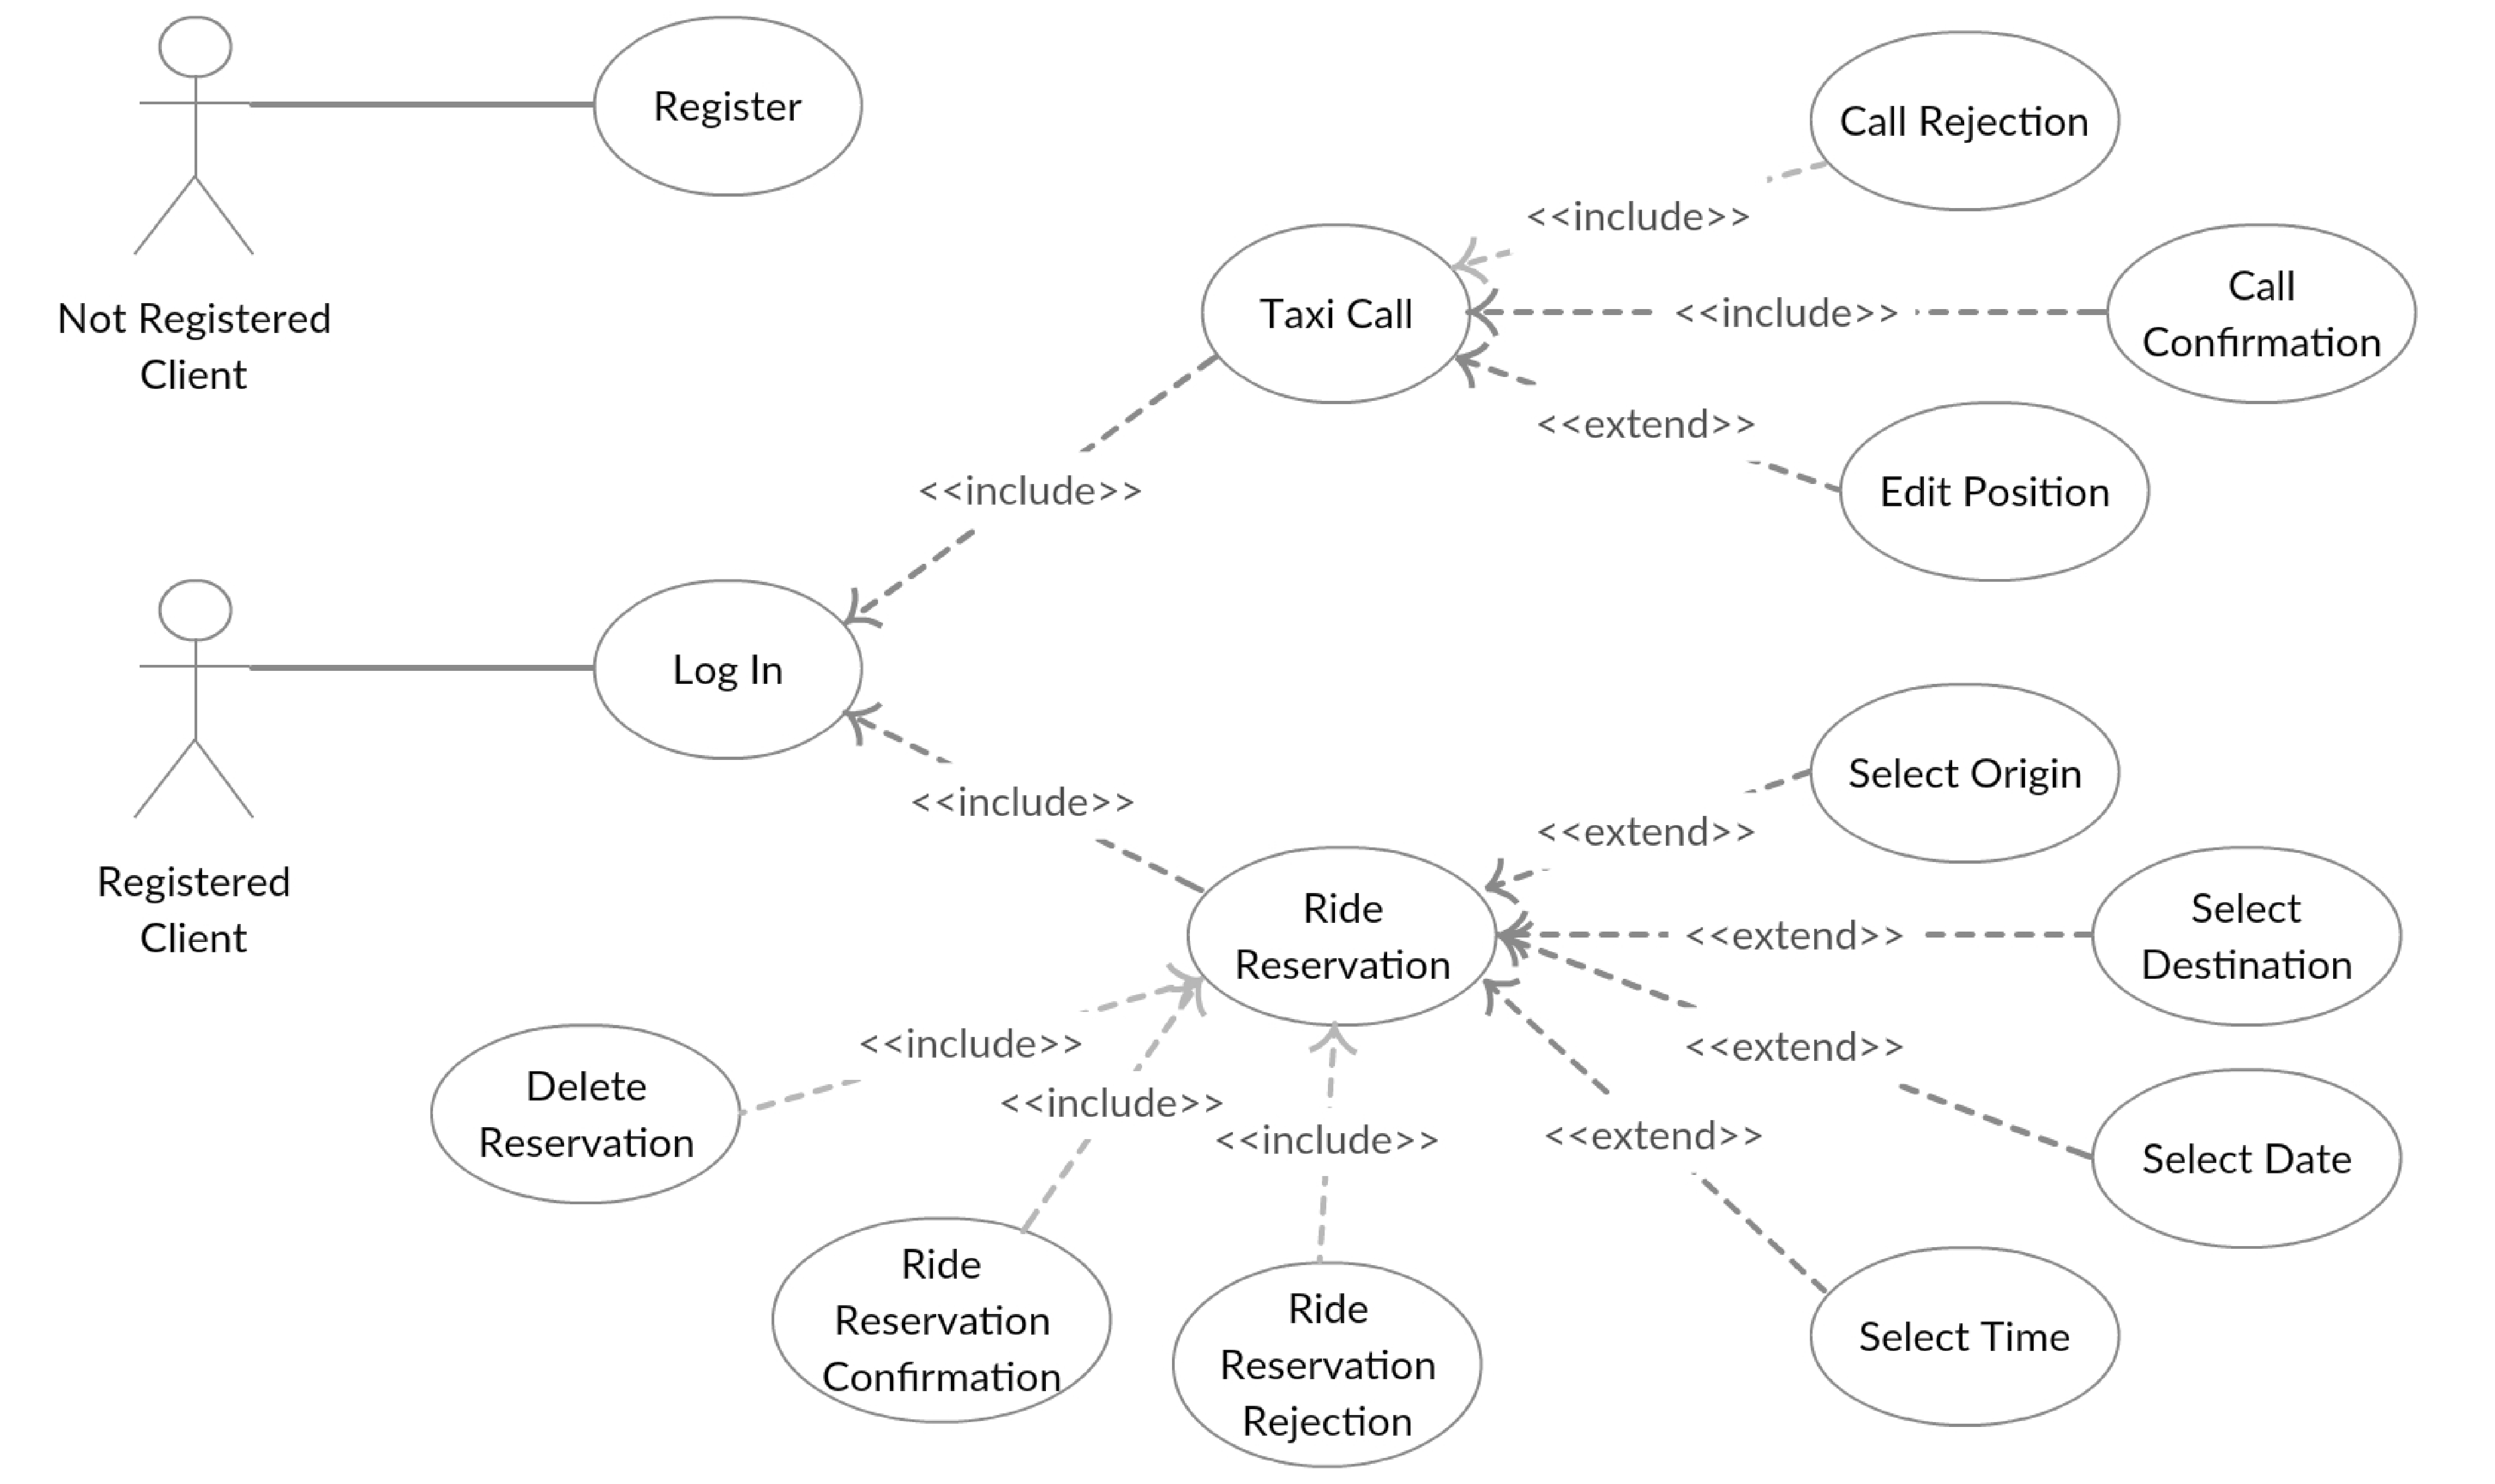
\includegraphics[width=\textwidth]{UseCase-Client}
\centering
\caption{Clients UML Use Case Diagrams}
\label{fig:usecaseclient}
\end{figure}

\vfill

\begin{figure}[H]
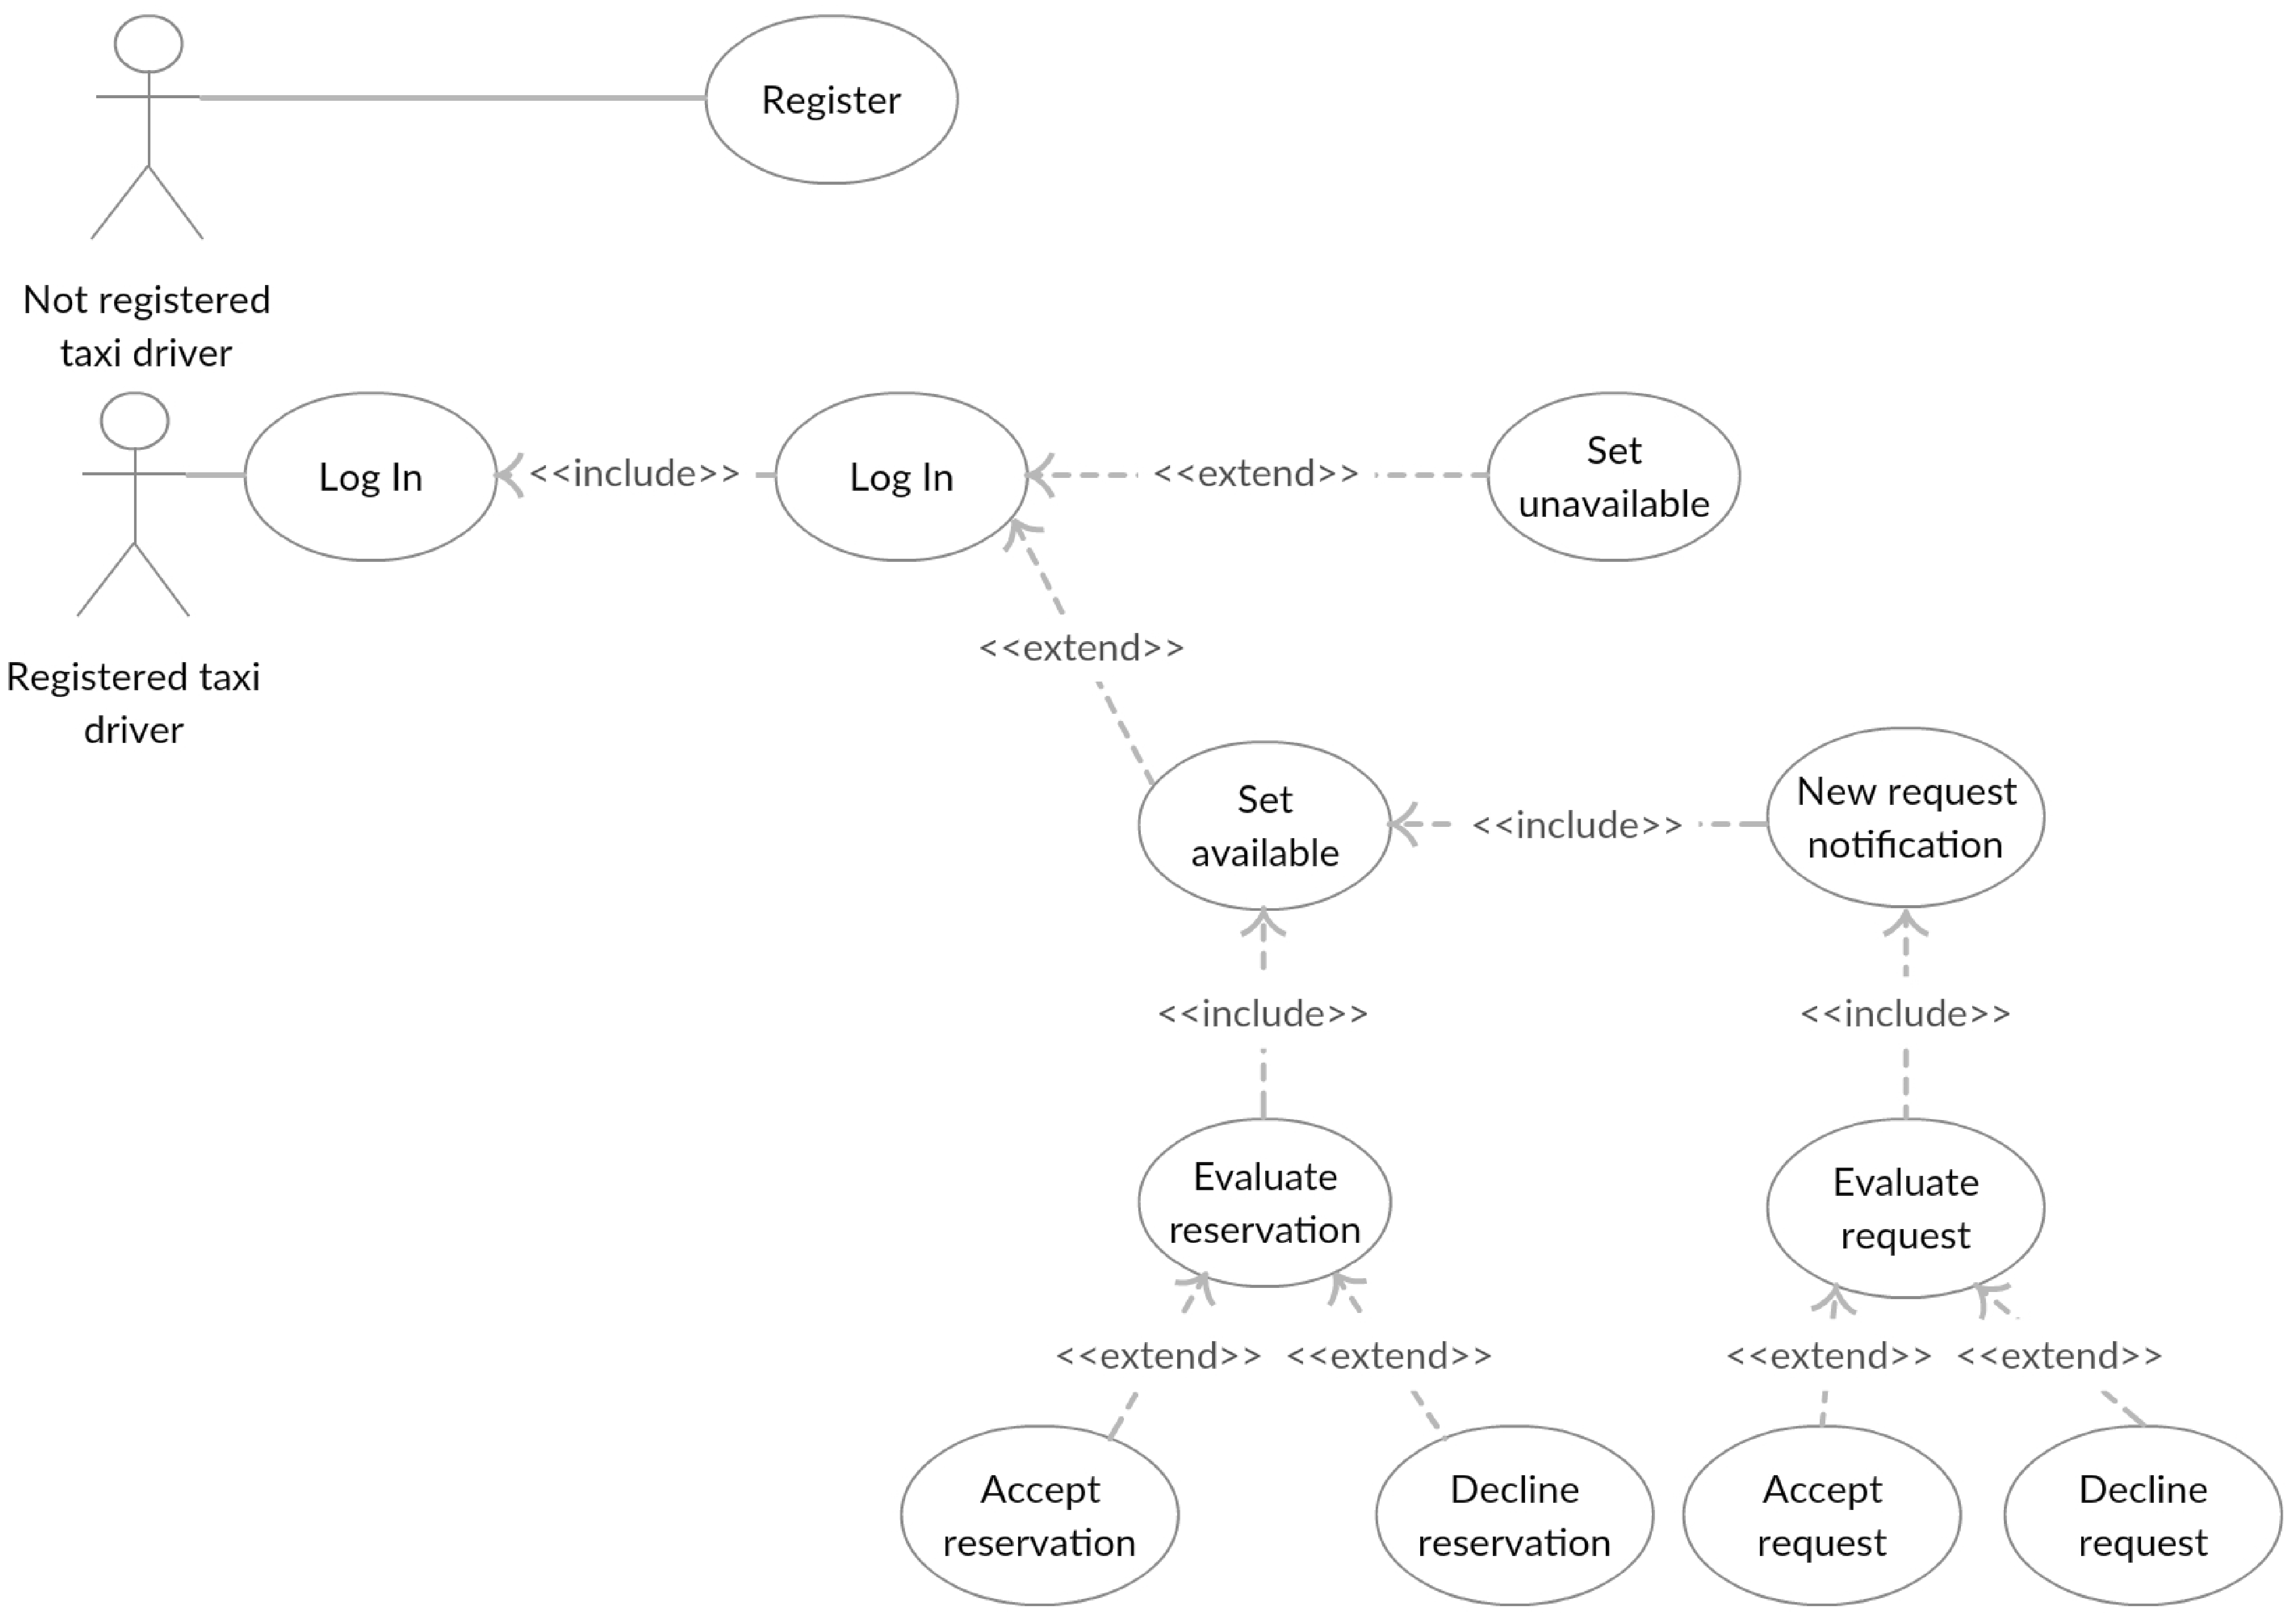
\includegraphics[width=\textwidth]{UseCase-TaxiDriver}
\centering
\caption{Taxi Drivers UML Use Case Diagrams}
\label{fig:usecasetaxidriver}
\end{figure}

\subsubsection{Use Case Descriptions}

% Increase the space between table's rows
\renewcommand{\arraystretch}{1.25}

\begin{table} [H]
\begin{center}
\begin{tabular}{ |m{.25\textwidth}|m{.65\textwidth}|  }
\hline
    \multicolumn{2}{|c|}{\textbf{\textit{Client Registration}}} \\
\hline \hline
    \textbf{Actors}
&   Not Registered Client
\\ \hline
    \textbf{Entry Conditions}
&   The Client is not registered to the service.
\\ \hline
    \textbf{Flow of Events}
& 
    \begin{enumerate*}
    \item The client browses to the website or opens the mobile app
    \item The client clicks on the \emph{REGISTER} button
    \item The client inputs the following data:
        \begin{enumerate*}
        \item e-mail address
        \item First Name
        \item Last Name
        \item Date of birth
        \item Phone Number
        \item Password
        \end{enumerate*}
    \item The client clicks on the \emph{Sign Up!} button
    \end{enumerate*}
\\ \hline
    \textbf{Exit Conditions}
&   Client is successfully registered and the login page will be shown. 

    Now they can log in and using e-mail and password inserted before.
\\ \hline
    \textbf{Exceptions}
&   
    An error will be shown if:
    \begin{itemize*}
    \item some field is empty
    \item e-mail already in use
    \item password is not long enough
    \item date of birth identifies an underage person
    \end{itemize*}
    The application will go back to the \emph{point 3} of the \emph{Flow of Events}
\\ \hline
\end{tabular}
\end{center}
\caption{Use Case Description of Client Registration}
\label{table:clientregistration}
\end{table}


\begin{table} [H]
\begin{center}
\begin{tabular}{ |m{.25\textwidth}|m{.65\textwidth}|  }
\hline
    \multicolumn{2}{|c|}{\textbf{\textit{Taxi Driver Registration}}} \\
\hline \hline
    \textbf{Actors}
&   Not Registered Taxi Driver
\\ \hline
    \textbf{Entry Conditions}
&   The Taxi Driver is not registered to the service.
\\ \hline
    \textbf{Flow of Events}
& 
    \begin{enumerate*}
    \item The driver open the mobile app
    \item The driver clicks on the \emph{REGISTER} button
    \item The driver inputs the following data:
        \begin{enumerate*}
        \item e-mail address
        \item First Name
        \item Last Name
        \item Phone Number
        \item License Number
        \item Password
        \end{enumerate*}
    \item The driver clicks on the \emph{Sign Up!} button
    \end{enumerate*}
\\ \hline
    \textbf{Exit Conditions}
&   Taxi Driver is successfully registered and the login page will be shown. 

    Now they can log in using e-mail and password inserted before.
\\ \hline
    \textbf{Exceptions}
&   
    An error will be shown if:
    \begin{itemize*}
    \item e-mail already in use
    \item password is not long enough
    \item invalid license number
    \end{itemize*}
    The application will go back to the \emph{point 3} of the \emph{Flow of Events} 
\\ \hline
\end{tabular}
\end{center}
\caption{Use Case Description of Taxi Driver Registration}
\label{table:taxiregistration}
\end{table}


\begin{table} [H]
\begin{center}
\begin{tabular}{ |m{.25\textwidth}|m{.65\textwidth}|  }
\hline
    \multicolumn{2}{|c|}{\textbf{\textit{Client Log in}}} \\
\hline \hline
    \textbf{Actors}
&   Registered Client
\\ \hline
    \textbf{Entry Conditions}
&   The Client must be registered to the service.
\\ \hline
    \textbf{Flow of Events}
& 
    \begin{enumerate*}
    \item The client browses to the website or open the mobile app
    \item The client clicks on the \emph{LOGIN} button
    \item The client inputs the following data:
        \begin{enumerate*}
        \item e-mail address
        \item Password
        \end{enumerate*}
    \item The client clicks on the \emph{Sign In!} button
    \end{enumerate*}
\\ \hline
    \textbf{Exit Conditions}
&   Client successfully logged in. 

    Now they can use the service.
\\ \hline
    \textbf{Exceptions}
&   
    An error will be shown if:
    \begin{itemize*}
    \item e-mail is wrong
    \item password is wrong
    The client can try to log in again.
    \end{itemize*}
    The client can try to log in again.
\\ \hline
\end{tabular}
\end{center}
\caption{Use Case Description of Client Log In}
\label{table:clientlogin}
\end{table}


\begin{table} [H]
\begin{center}
\begin{tabular}{ |m{.25\textwidth}|m{.65\textwidth}|  }
\hline
    \multicolumn{2}{|c|}{\textbf{\textit{Taxi Driver Log in}}} \\
\hline \hline
    \textbf{Actors}
&   Registered Taxi Driver
\\ \hline
    \textbf{Entry Conditions}
&   The Taxi Driver must be registered to the service.
\\ \hline
    \textbf{Flow of Events}
& 
    \begin{enumerate*}
    \item The driver opens the mobile app
    \item The driver clicks on the \emph{LOGIN} button
    \item The driver inputs the following data:
        \begin{enumerate*}
        \item e-mail address
        \item Password
        \end{enumerate*}
    \item The driver clicks on the \emph{Sign In!} button
    \end{enumerate*}
\\ \hline
    \textbf{Exit Conditions}
&   Driver successfully logged in.

    Now they can use the service.
\\ \hline
    \textbf{Exceptions}
&   
    An error will be shown if:
    \begin{itemize*}
    \item e-mail is wrong
    \item password is wrong
    \end{itemize*}
    The driver can try to log in again.
\\ \hline
\end{tabular}
\end{center}
\caption{Use Case Description of Taxi Driver Log In}
\label{table:taxilogin}
\end{table}

\begin{table} [H]
\begin{center}
\begin{tabular}{ |m{.25\textwidth}|m{.65\textwidth}|  }
\hline
    \multicolumn{2}{|c|}{\textbf{\textit{Client makes a Taxi Call}}} \\
\hline \hline
    \textbf{Actors}
&   Registered Client
\\ \hline
    \textbf{Entry Conditions}
&   The Client must be logged into the website or the application.
\\ \hline
    \textbf{Flow of Events}
& 
    \begin{enumerate*}
    \item The client clicks on the \emph{Taxi Call} button in the menu
    \item The app (or website) shows the current position of the user retrieved by the GPS
    \item The client can modify the position
    \item The client clicks on the \emph{Call a Taxi!} button
    \end{enumerate*}
\\ \hline
    \textbf{Exit Conditions}
&   The call is successfully forwarded to the system.
\\ \hline
    \textbf{Exceptions}
&   
    There are not exceptions for this use case.
\\ \hline
\end{tabular}
\end{center}
\caption{Use Case Description of a Taxi Call}
\label{table:clientcall}
\end{table}

\begin{table} [H]
\begin{center}
\begin{tabular}{ |m{.25\textwidth}|m{.65\textwidth}|  }
\hline
    \multicolumn{2}{|c|}{\textbf{\textit{The client receives a Taxi Call Confirmation}}} \\
\hline \hline
    \textbf{Actors}
&   Registered Client
\\ \hline
    \textbf{Entry Conditions}
&   The Client must be logged into the website or the application.
\\ \hline
    \textbf{Flow of Events}
& 
    \begin{enumerate*}
    \item The client receives a notification
    \item The app (or website) shows the number of the taxi which will arrive, the taxi driver's phone number and the waiting time
    \end{enumerate*}
\\ \hline
    \textbf{Exit Conditions}
&   The call will arrive in the specified waiting time.
\\ \hline
    \textbf{Exceptions}
&   
    There are not exceptions for this use case.
\\ \hline
\end{tabular}
\end{center}
\caption{Use Case Description of a Taxi Call Confirmation}
\label{table:clientconfirmation}
\end{table}

\begin{table} [H]
\begin{center}
\begin{tabular}{ |m{.25\textwidth}|m{.65\textwidth}|  }
\hline
    \multicolumn{2}{|c|}{\textbf{\textit{The client receives a Taxi Call Rejection}}} \\
\hline \hline
    \textbf{Actors}
&   Registered Client
\\ \hline
    \textbf{Entry Conditions}
&   The Client must be logged into the website or the application.
\\ \hline
    \textbf{Flow of Events}
& 
    \begin{enumerate*}
    \item The client receives a notification
    \item The app (or website) shows that their request was rejected
    \end{enumerate*}
\\ \hline
    \textbf{Exit Conditions}
&   The client is able to make another call.
\\ \hline
    \textbf{Exceptions}
&   
    There are not exceptions for this use case.
\\ \hline
\end{tabular}
\end{center}
\caption{Use Case Description of a Taxi Call Rejection}
\label{table:clientrejection}
\end{table}


\begin{table} [H]
\begin{center}
\begin{tabular}{ |m{.25\textwidth}|m{.65\textwidth}|  }
\hline
    \multicolumn{2}{|c|}{\textbf{\textit{The client makes a Ride Reservation }}} \\
\hline \hline
    \textbf{Actors}
&   Registered Client
\\ \hline
    \textbf{Entry Conditions}
&   The Client must be logged into the website or the application.
\\ \hline
    \textbf{Flow of Events}
& 
    \begin{enumerate*}
    \item The client clicks on the \emph{Ride Reservation} button in the menu
    \item The client has to set the following parameters
        \begin{enumerate*}
        \item Origin
        \item Destination
        \item Date
        \item Time
        \end{enumerate*}
    \item The client clicks on the \emph{Reserve a Ride!} button
    \end{enumerate*}
\\ \hline
    \textbf{Exit Conditions}
&   The reservation request is forwarded to the system.
\\ \hline
    \textbf{Exceptions}
&   An error will be shown if:
    \begin{itemize*}
    \item the origin is out of the city
    \item the date is in the past
    \item the selected time is not at least two hours after the current time
    \end{itemize*}
\\ \hline
\end{tabular}
\end{center}
\caption{Use Case Description of a Ride Reservation}
\label{table:clientridereservation}
\end{table}

\begin{table} [H]
\begin{center}
\begin{tabular}{ |m{.25\textwidth}|m{.65\textwidth}|  }
\hline
    \multicolumn{2}{|c|}{\textbf{\textit{The client deletes a Ride Reservation }}} \\
\hline \hline
    \textbf{Actors}
&   Registered Client
\\ \hline
    \textbf{Entry Conditions}
&   The Client must be logged into the website or the application.
\\ \hline
    \textbf{Flow of Events}
& 
    \begin{enumerate*}
    \item The client clicks on the \emph{Your Reservations} button in the menu
    \item The client clicks on the reservation who wants to delete from the list
    \item The application shows the reservation's details
    \item The client clicks on the \emph{Delete} button
    \end{enumerate*}
\\ \hline
    \textbf{Exit Conditions}
&   The reservation was successfully deleted.
\\ \hline
    \textbf{Exceptions}
&   The client cannot delete the reservation if the meeting time is sooner than ten minutes.
\\ \hline
\end{tabular}
\end{center}
\caption{Use Case Description of a Client who deletes a Ride Reservation}
\label{table:clientdeleteridereservation}
\end{table}

\begin{table} [H]
\begin{center}
\begin{tabular}{ |m{.25\textwidth}|m{.65\textwidth}|  }
\hline
    \multicolumn{2}{|c|}{\textbf{\textit{The client receives a Ride Reservation Confirmation}}} \\
\hline \hline
    \textbf{Actors}
&   Registered Client
\\ \hline
    \textbf{Entry Conditions}
&   The Client must be logged into the website or the application.
\\ \hline
    \textbf{Flow of Events}
& 
    \begin{enumerate*}
    \item The client receives a notification
    \item The app (or website) shows the number of the taxi which will arrive, the taxi driver's phone number, the place and the meeting time.
    \end{enumerate*}
\\ \hline
    \textbf{Exit Conditions}
&   The taxi will arrive at the meeting place at the specified time.
\\ \hline
    \textbf{Exceptions}
&   
    There are not exceptions for this use case.
\\ \hline
\end{tabular}
\end{center}
\caption{Use Case Description of a Ride Reservation Confirmation}
\label{table:clientrideconfirmation}
\end{table}

\begin{table} [H]
\begin{center}
\begin{tabular}{ |m{.25\textwidth}|m{.65\textwidth}|  }
\hline
    \multicolumn{2}{|c|}{\textbf{\textit{The client receives a Ride Reservation Rejection}}} \\
\hline \hline
    \textbf{Actors}
&   Registered Client
\\ \hline
    \textbf{Entry Conditions}
&   The Client must be logged into the website or the application.
\\ \hline
    \textbf{Flow of Events}
& 
    \begin{enumerate*}
    \item The client receives a notification
    \item The app (or website) shows that their ride request was rejected
    \end{enumerate*}
\\ \hline
    \textbf{Exit Conditions}
&   The client is able to make another call or reservation.
\\ \hline
    \textbf{Exceptions}
&   
    There are not exceptions for this use case.
\\ \hline
\end{tabular}
\end{center}
\caption{Use Case Description of a Ride Reservation Rejection}
\label{table:clienridetrejection}
\end{table}


\begin{table} [H]
\begin{center}
\begin{tabular}{ |m{.25\textwidth}|m{.65\textwidth}|  }
\hline
    \multicolumn{2}{|c|}{\textbf{\textit{Taxi Driver changes their availability state}}} \\
\hline \hline
    \textbf{Actors}
&   Registered Taxi Driver
\\ \hline
    \textbf{Entry Conditions}
&   The Taxi Driver must be logged into the application.
\\ \hline
    \textbf{Flow of Events}
& 
    \begin{enumerate*}
    \item The driver opens the mobile app
    \item The driver clicks on the \emph{Change State} button
    \item The driver taps on the button relative to their state:
        \begin{itemize*}
        \item \emph{available}
        \item \emph{unavailable}
        \end{itemize*}
    \end{enumerate*}
\\ \hline
    \textbf{Exit Conditions}
&  The availability state will be updated and the application will come back to the home.
\\ \hline
    \textbf{Exceptions}
&   Nothing will happen if the driver tries to select the same state in which they were before.
\\ \hline
\end{tabular}
\end{center}
\caption{Use Case Description of Taxi Driver who changes their availability state}
\label{table:taxichangestate}
\end{table}

\begin{table} [H]
\begin{center}
\begin{tabular}{ |m{.25\textwidth}|m{.65\textwidth}|  }
\hline
    \multicolumn{2}{|c|}{\textbf{\textit{The Taxi Driver receives a new call request notification}}} \\
\hline \hline
    \textbf{Actors}
&   Registered Taxi Driver
\\ \hline
    \textbf{Entry Conditions}
&   
    \begin{itemize*}
    \item The Taxi Driver must be logged into the application
    \item The application must be opened or running in background
    \item The Taxi Driver state must be \emph{Available}
    \end{itemize*}
\\ \hline
    \textbf{Flow of Events}
& 
    \begin{enumerate*}
    \item The driver smartphone rings or vibrates (according to user's settings)
    \item The driver clicks on the notification
    \item The app shows the details of the incoming call:
        \begin{itemize*}
        \item Client Position
        \item Client Phone Number
        \end{itemize*}
    \end{enumerate*}
\\ \hline
    \textbf{Exit Conditions}
&  The applications is showing the details and the taxi driver has to evaluate this request.
\\ \hline
    \textbf{Exceptions}
&   There are not exceptions for this use case.
\\ \hline
\end{tabular}
\end{center}
\caption{Use Case Description of Taxi Driver who receives a call notification}
\label{table:taxireceivenotification}
\end{table}

\begin{table} [H]
\begin{center}
\begin{tabular}{ |m{.25\textwidth}|m{.65\textwidth}|  }
\hline
    \multicolumn{2}{|c|}{\textbf{\textit{The Taxi Driver evaluates a call request}}} \\
\hline \hline
    \textbf{Actors}
&   Registered Taxi Driver
\\ \hline
    \textbf{Entry Conditions}
&   
    \begin{itemize*}
    \item The Taxi Driver must be logged into the application
    \item The Taxi Driver must have received a request notification
    \item The application must be opened on the call request
    \end{itemize*}
\\ \hline
    \textbf{Flow of Events}
& 
    \begin{enumerate*}
    \item The driver smartphone shows the details of the incoming call
    \item The Taxi Driver clicks on \emph{Accept} button
    \end{enumerate*}
\\ \hline
    \textbf{Exit Conditions}
&  The Taxi Driver has to go to take their client who has received the confirmation.
\\ \hline
    \textbf{Exceptions}
&   If the taxi driver clicks on \emph{Decline} or the timeout runs out, the request will pass to the next driver present in the queue. \newline
If the queue is ended, the client will receive a call rejection notification.
\\ \hline
\end{tabular}
\end{center}
\caption{Use Case Description of Taxi Driver who decides to accept or decline a call request}
\label{table:taxievaluateriderequest}
\end{table}

\begin{table} [H]
\begin{center}
\begin{tabular}{ |m{.25\textwidth}|m{.65\textwidth}|  }
\hline
    \multicolumn{2}{|c|}{\textbf{\textit{The Taxi Driver receives a new ride reservation request notification}}} \\
\hline \hline
    \textbf{Actors}
&   Registered Taxi Driver
\\ \hline
    \textbf{Entry Conditions}
&   
    \begin{itemize*}
    \item The Taxi Driver must be logged into the application
    \item The application must be opened or running in background
    \end{itemize*}
\\ \hline
    \textbf{Flow of Events}
& 
    \begin{enumerate*}
    \item The driver smartphone rings or vibrates (according to user's settings)
    \item The driver clicks on the notification
    \item The app shows the details of the ride reservation request:
        \begin{itemize*}
        \item Origin
        \item Destination
        \item Date
        \item Time
        \item Client Phone Number
        \end{itemize*}
    \end{enumerate*}
\\ \hline
    \textbf{Exit Conditions}
&  The applications is showing the details and the taxi driver has to evaluate this request.
\\ \hline
    \textbf{Exceptions}
&   There are not exceptions for this use case.
\\ \hline
\end{tabular}
\end{center}
\caption{Use Case Description of Taxi Driver who receives a call notification}
\label{table:taxireceiveridereservationnotification}
\end{table}

\begin{table} [H]
\begin{center}
\begin{tabular}{ |m{.25\textwidth}|m{.65\textwidth}|  }
\hline
    \multicolumn{2}{|c|}{\textbf{\textit{The Taxi Driver evaluates a Ride Reservarion request}}} \\
\hline \hline
    \textbf{Actors}
&   Registered Taxi Driver
\\ \hline
    \textbf{Entry Conditions}
&   
    \begin{itemize*}
    \item The Taxi Driver must be logged into the application
    \item The Taxi Driver must have received a request notification
    \item The application must be opened on the ride reservation request
    \end{itemize*}
\\ \hline
    \textbf{Flow of Events}
& 
    \begin{enumerate*}
    \item The driver smartphone shows the details of the ride
    \item The Taxi Driver clicks on \emph{Accept} button
    \end{enumerate*}
\\ \hline
    \textbf{Exit Conditions}
&  The Taxi Driver has to go to take their client who has received the confirmation.
\\ \hline
    \textbf{Exceptions}
&   If the taxi driver clicks on \emph{Decline} or the timeout runs out, the request will pass to the next driver in the system \newline
If all the taxi drivers have declined the request, a rejection will be sent to the client
\\ \hline
\end{tabular}
\end{center}
\caption{Use Case Description of Taxi Driver who decides to accept or decline a Ride Reservation request}
\label{table:taxievaluaterequest}
\end{table}

\subsubsection{Use Case Sequence Diagrams}

% Sequences Width
\newlength{\sequenceWidth}
\setlength{\sequenceWidth}{\textwidth}

\begin{figure}[H]
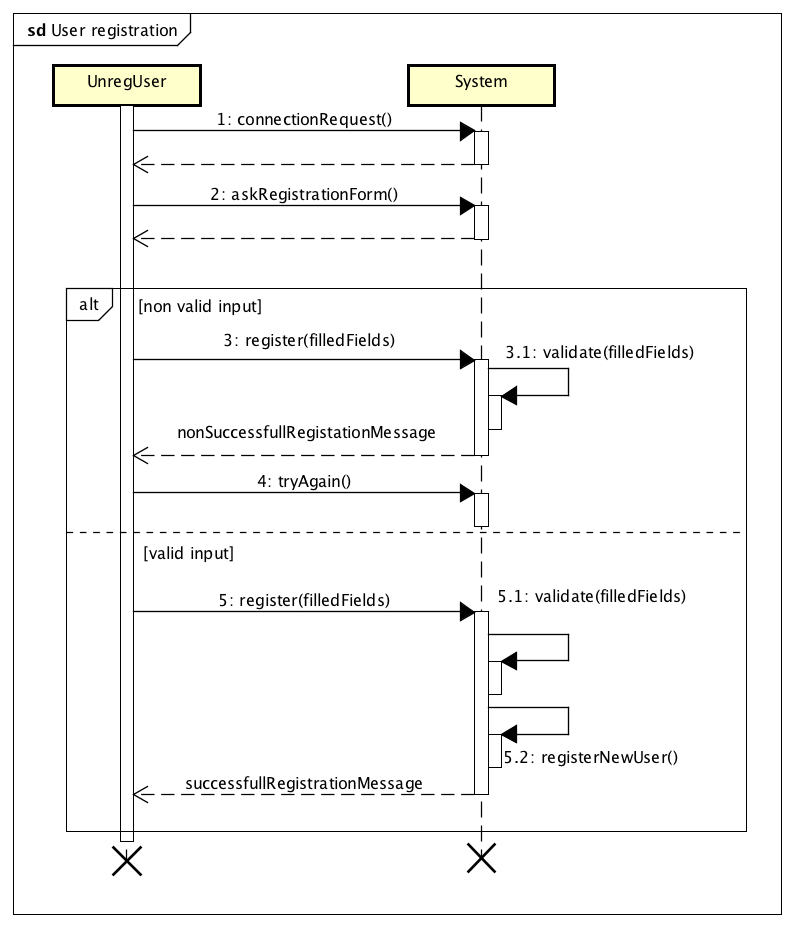
\includegraphics[width=\sequenceWidth]{Sequence-Client-Registration}
\centering
\caption{Client Registration UML Sequence Diagram}
\label{fig:sequenceclientregistration}
\end{figure}

\begin{figure}[H]
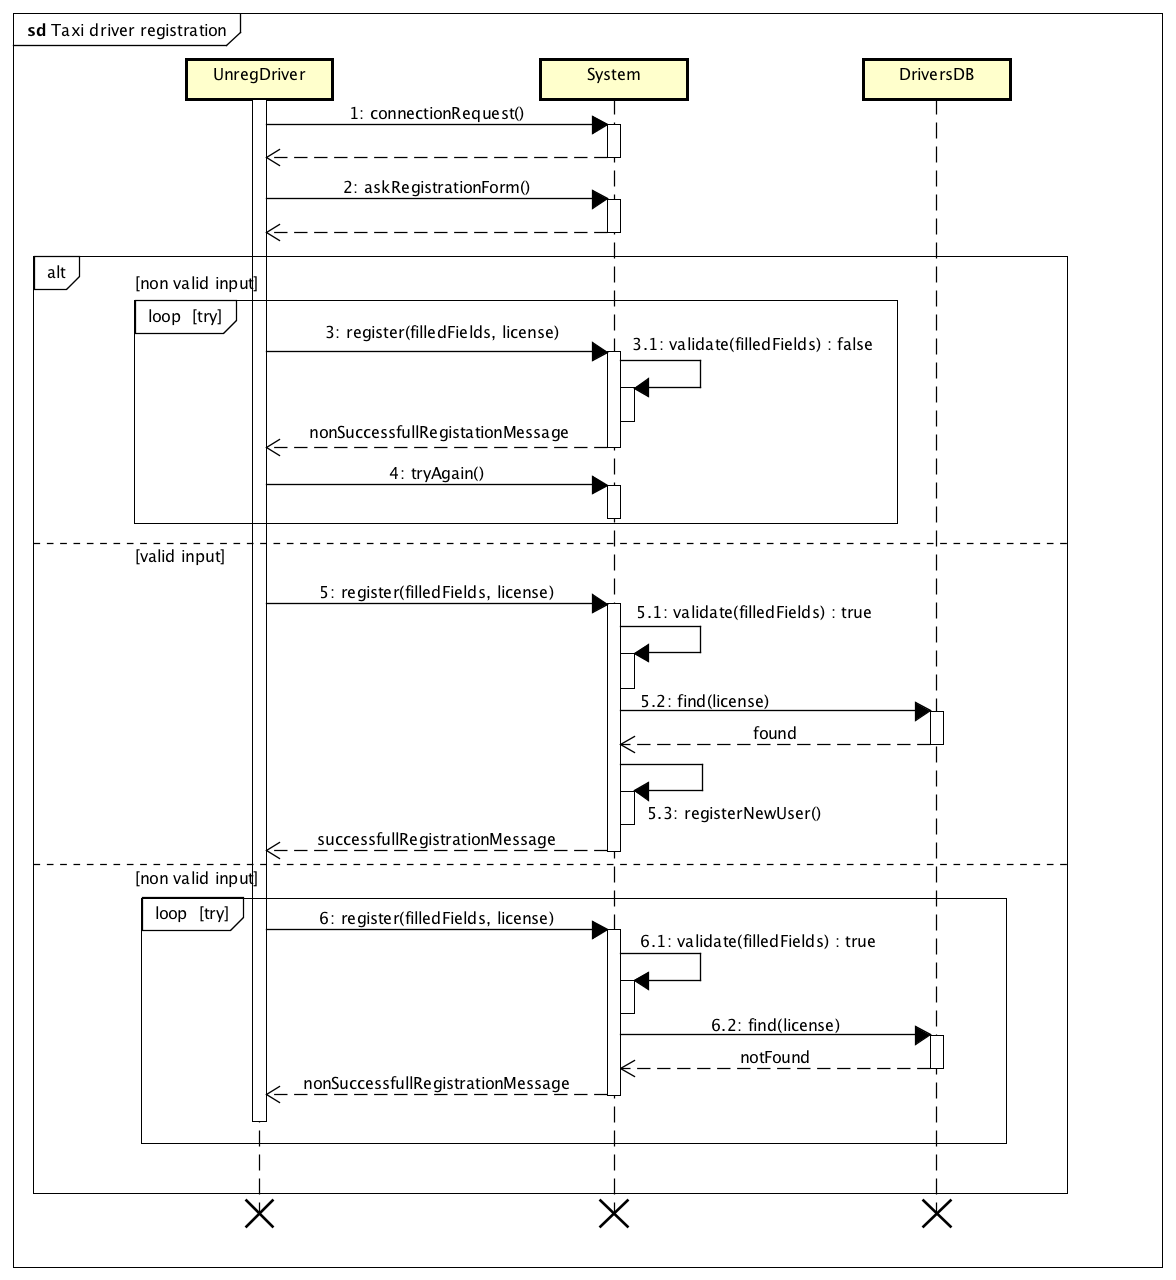
\includegraphics[width=\sequenceWidth]{Sequence-TaxiDriver-Registration}
\centering
\caption{Taxi Driver UML Sequence Diagram}
\label{fig:sequencetaxidriverregistration}
\end{figure}

\begin{figure}[H]
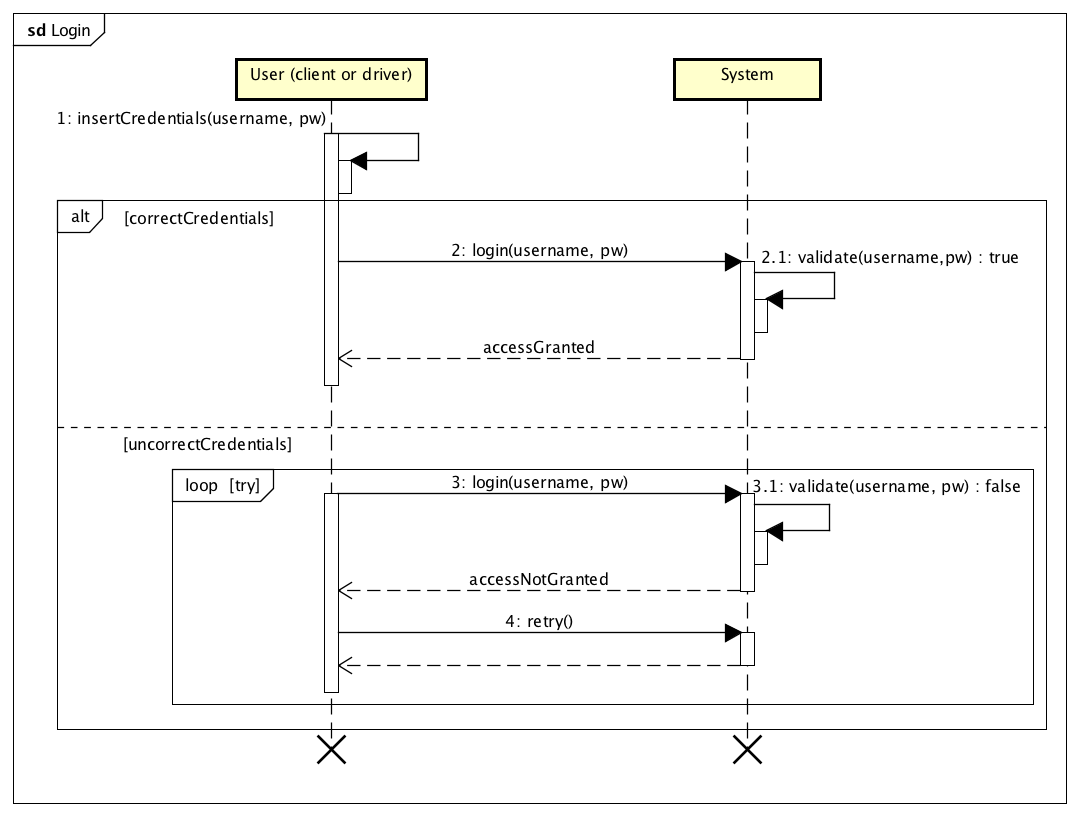
\includegraphics[width=\sequenceWidth]{Sequence-Login}
\centering
\caption{Login Sequence Diagram}
\label{fig:sequencelogin}
\end{figure}

\begin{figure}[H]
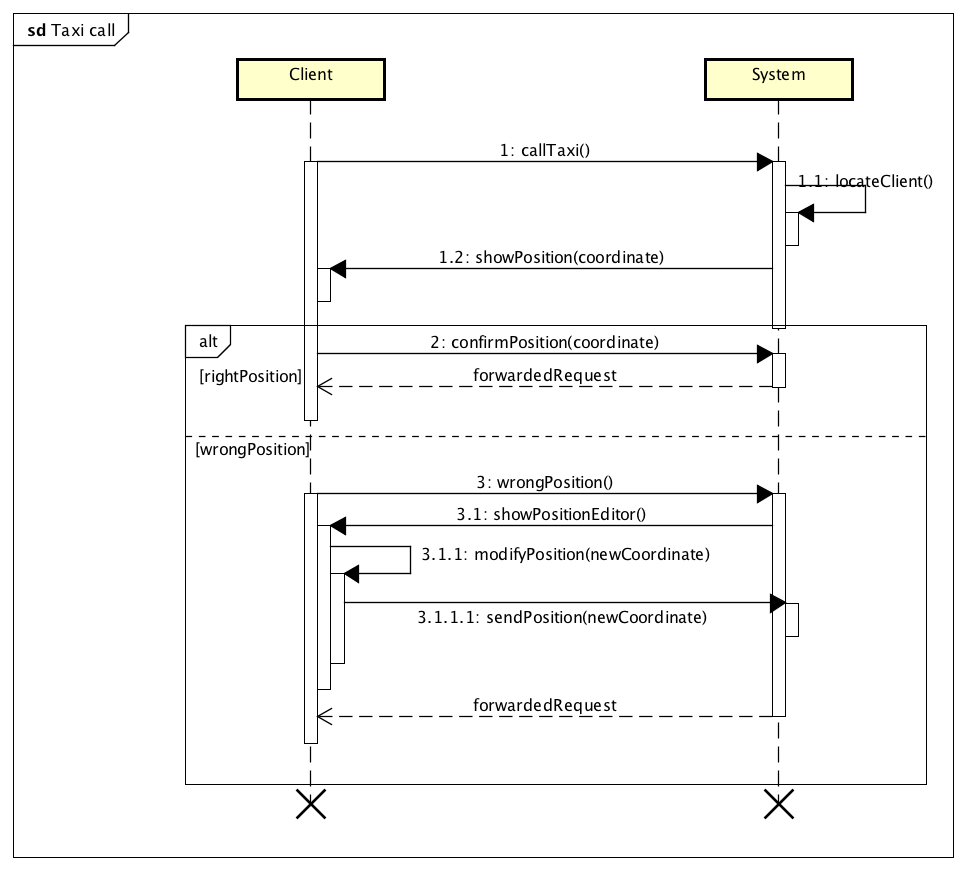
\includegraphics[width=\sequenceWidth]{Sequence-Client-TaxiCall}
\centering
\caption{Client Taxi Call UML Sequence Diagram}
\label{fig:sequenceclienttaxicall}
\end{figure}

\begin{figure}[H]
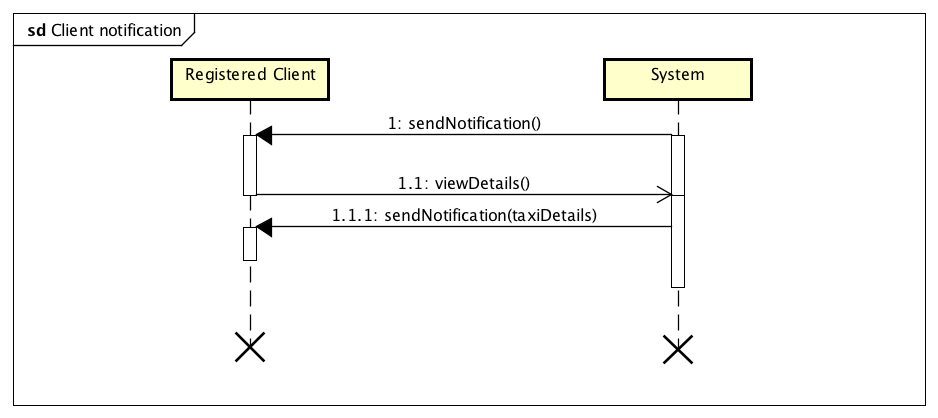
\includegraphics[width=\sequenceWidth]{Sequence-Client-Notification}
\centering
\caption{Client Call Confirmation UML Sequence Diagram}
\label{fig:sequenceclientnotification}
\end{figure}

\begin{figure}[H]
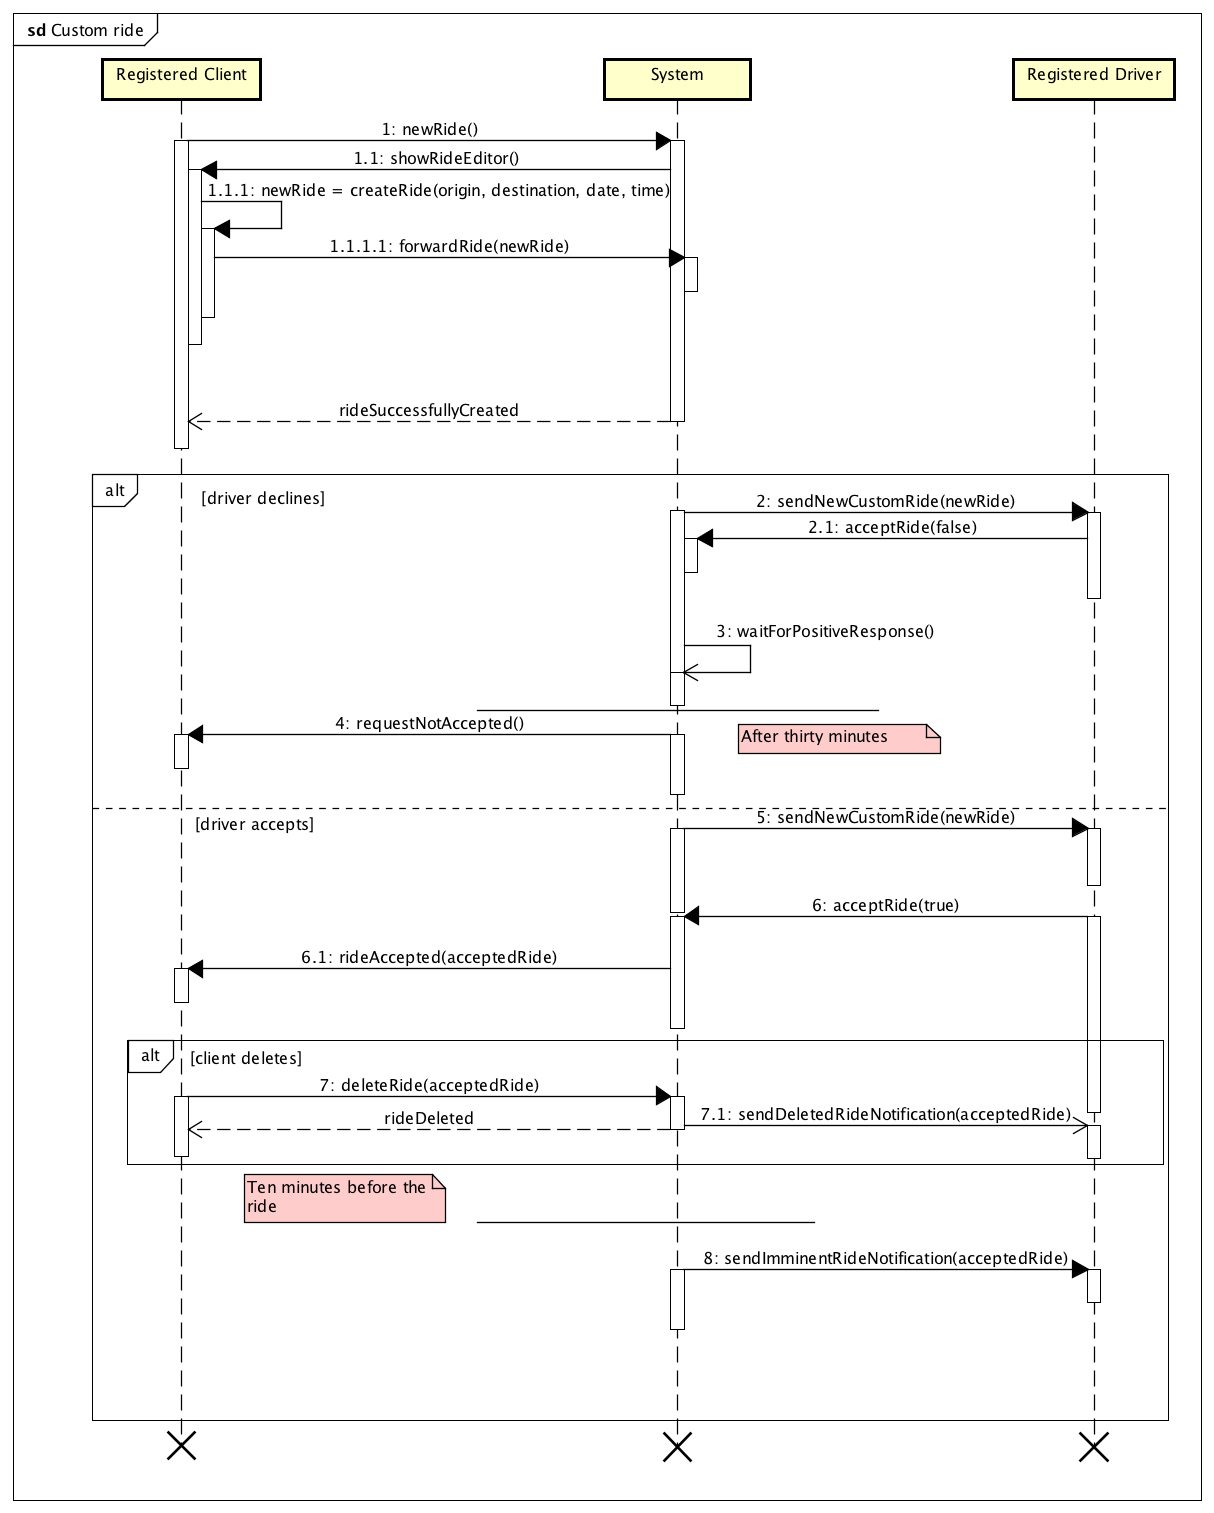
\includegraphics[width=\sequenceWidth]{Sequence-Client-RideReservation}
\centering
\caption{Client Ride Reservation and Driver accepts/declines UML Sequence Diagram}
\label{fig:sequenceclientridereservation}
\end{figure}

\begin{figure}[H]
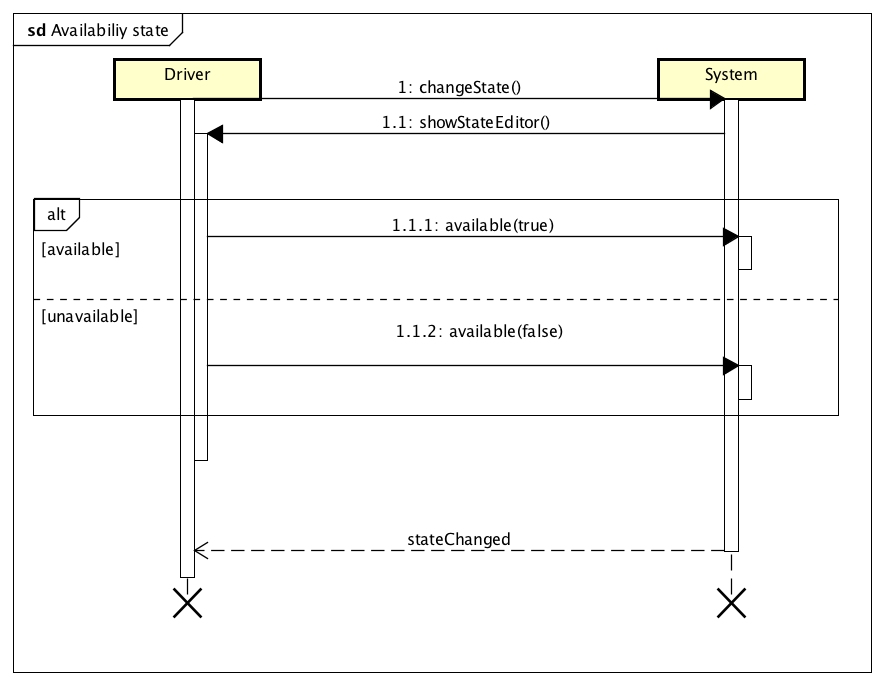
\includegraphics[width=\sequenceWidth]{Sequence-TaxiDriver-ChangeAvailabilityState}
\centering
\caption{Taxi Driver Change Availability State UML Sequence Diagram}
\label{fig:sequencetaxidriverchangestate}
\end{figure}

\begin{figure}[H]
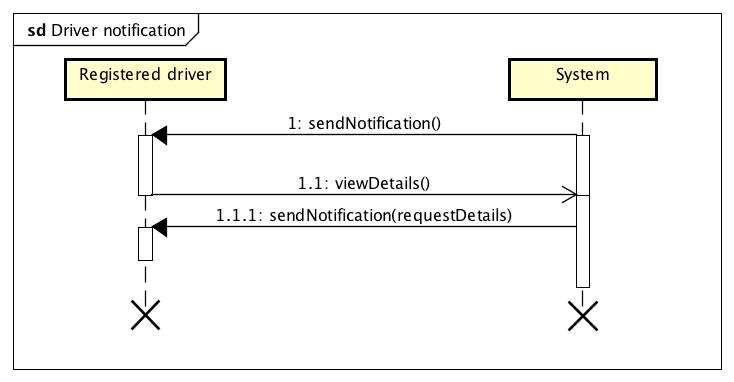
\includegraphics[width=\sequenceWidth]{Sequence-TaxiDriver-Notification}
\centering
\caption{Taxi Driver Request Notification UML Sequence Diagram}
\label{fig:sequencetaxidrivernotification}
\end{figure}

\begin{figure}[H]
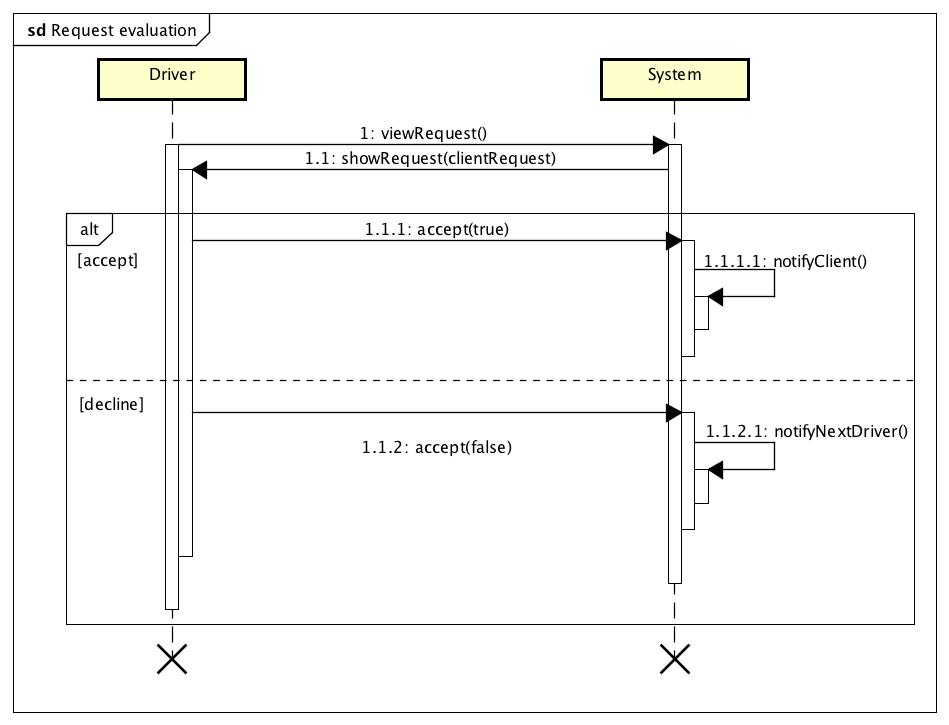
\includegraphics[width=\sequenceWidth]{Sequence-TaxiDriver-RequestEvaluation}
\centering
\caption{Taxi Driver Request Evaluation UML Sequence Diagram}
\label{fig:sequencetaxidriverrequestevaluation}
\end{figure}

\subsubsection{BPMN Diagrams}

\begin{figure}[H]
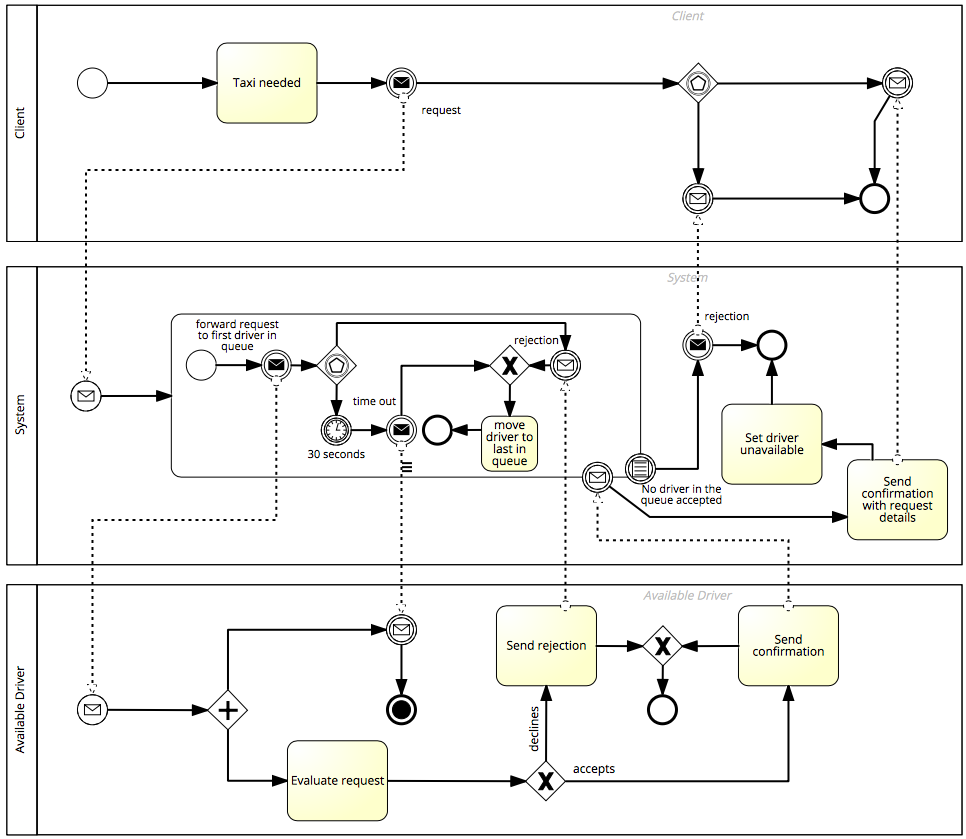
\includegraphics[width=\sequenceWidth]{BPMN-rideRequest}
\centering
\caption[BPMN Taxi Call]{This is a BPMN diagram of the taxi's request process of \emph{myTaxiService}}
\label{fig:bpmndiagramrequest}
\end{figure}

\begin{figure}[H]
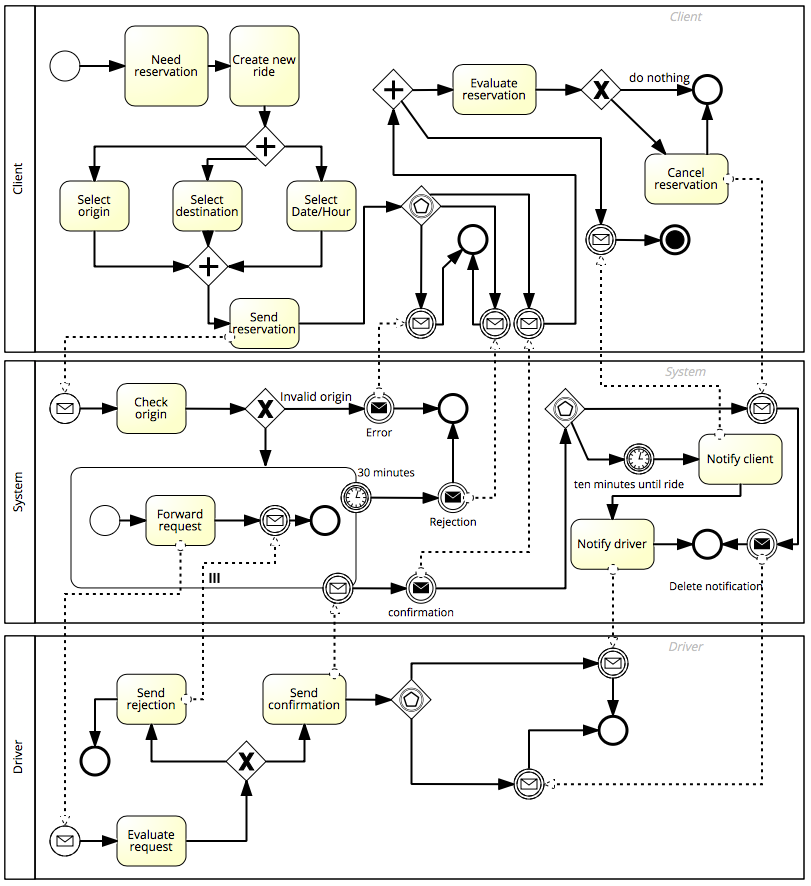
\includegraphics[width=\sequenceWidth]{BPMN-rideReservation}
\centering
\caption[BPMN Ride Reservation]{This is a BPMN diagram of the taxi's reservation process of \emph{myTaxiService}}
\label{fig:bpmndiagramreservation}
\end{figure}


\subsubsection{Class Diagram}

\begin{figure}[H]
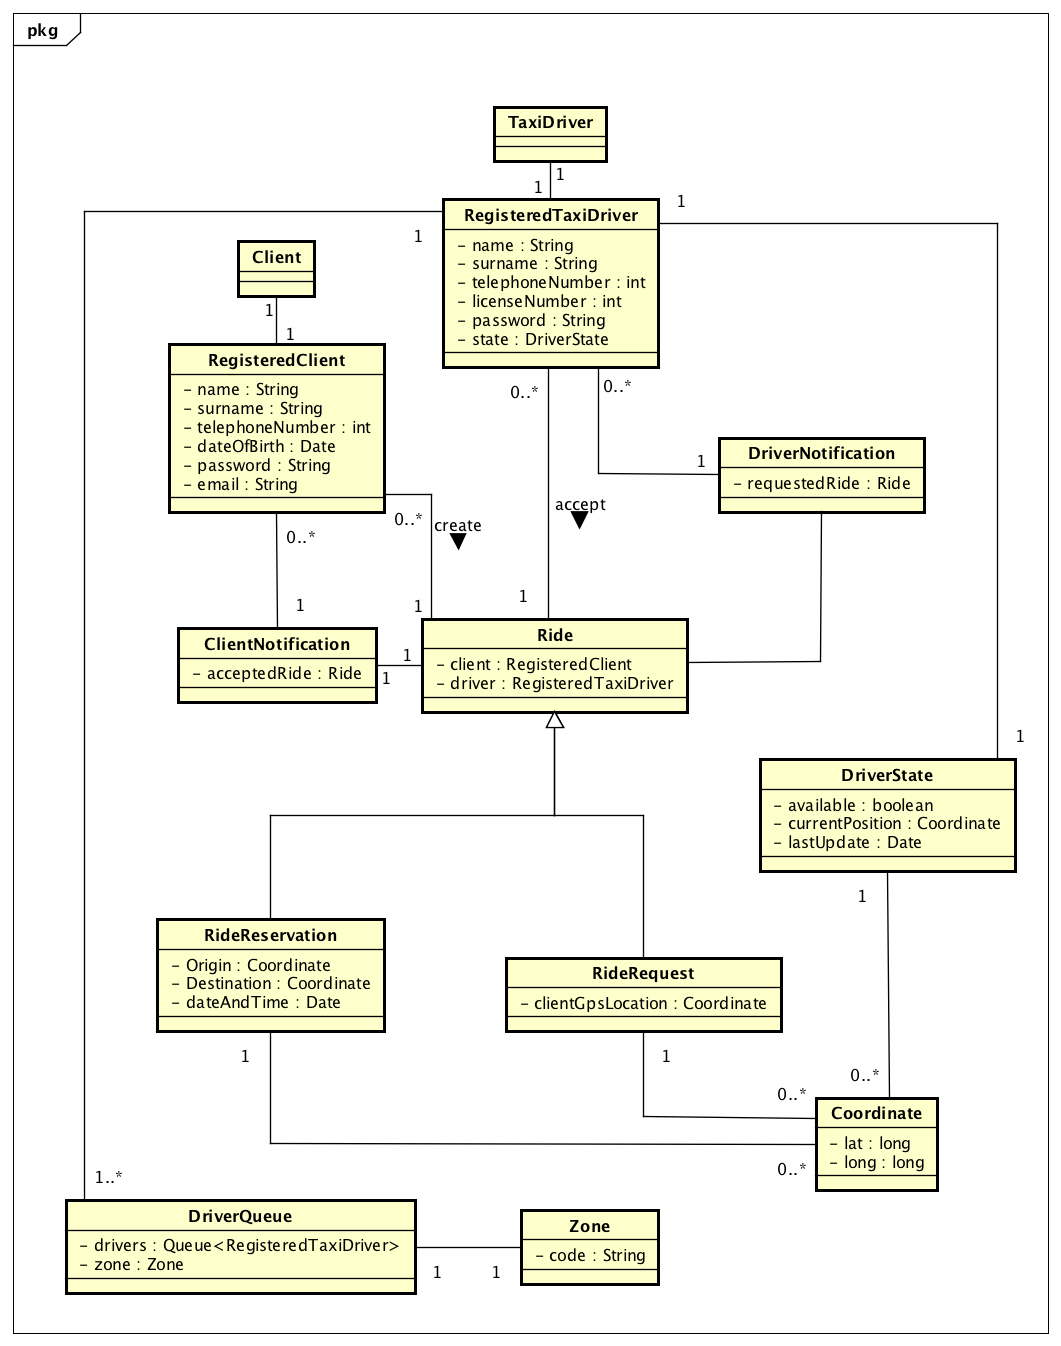
\includegraphics[width=\sequenceWidth]{ClassDiagramMyTaxiService}
\centering
\caption[UML Class Diagram]{This is an high level class diagram of \emph{myTaxiService}}
\label{fig:classdiagram}
\end{figure}

\section{Appendixes}

\subsection{Alloy}

We have used the \emph{Alloy Analyzer} in our project to make a formal definition of the most important properties of our system. In the following sections the model and the results derived using this tool are presented.

\newlength{\codeWidth}
\setlength{\codeWidth}{\textwidth}

\subsubsection{Signatures}

Here are presented the signatures of our model. Some fields which have not a relevant importance in term of constraint were omitted in order to make the model as simpler as possible.

\nopagebreak
\begin{minipage}[c]{\codeWidth}
\lstinputlisting[language=alloy]{alloy/signatures.als}
\end{minipage}

\subsubsection{Facts}

In this section the code represent all the constraints necessary to make the model consistent.

\nopagebreak
\begin{minipage}[c]{\codeWidth}
\lstinputlisting[language=alloy]{alloy/facts.als}
\end{minipage}


\subsubsection{Functions}

The following code is a function used to write assertions in an easy way.

\nopagebreak
\begin{minipage}[c]{\codeWidth}
\lstinputlisting[language=alloy]{alloy/functions.als}
\end{minipage}

\subsubsection{Assertions}

Here there are some assertions to be checked in order to verify the model.

\nopagebreak
\begin{minipage}[c]{\codeWidth}
\lstinputlisting[language=alloy]{alloy/assertions.als}
\end{minipage}

\subsubsection{Predicates}

The code below is the declaration of some predicates.

\nopagebreak
\begin{minipage}[c]{\codeWidth}
\lstinputlisting[language=alloy]{alloy/predicates.als}
\end{minipage}

\subsubsection{Main}

This is the main code of the model.

\nopagebreak
\begin{minipage}[c]{\codeWidth}
\lstinputlisting[language=alloy]{alloy/main.als}
\end{minipage}

\subsubsection{Output}

The following screenshot represents the output generated by the \emph{Alloy Analyzer} starting from the code presented in the previous sections. It shows that the model is consistent.

\nopagebreak
\begin{figure}[H]
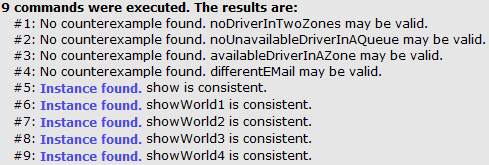
\includegraphics[width=.7\textwidth]{Alloy-Output}
\centering
\caption{Alloy Output}
\label{fig:alloyoutput}
\end{figure}

\subsubsection{Worlds}

The images in this section represent some \emph{Worlds} generated with \emph{Alloy Analyzer}. These \emph{Worlds} show some configurations of our system.

\newlength{\worldsWidth}
\setlength{\worldsWidth}{.9\textwidth}

\nopagebreak
\begin{figure}[H]
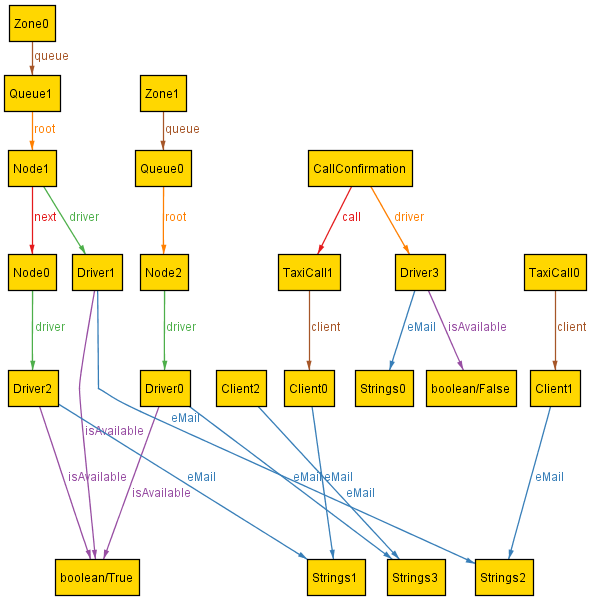
\includegraphics[width=\worldsWidth]{Alloy-Generic}
\centering
\caption[Alloy Generic World]{This alloy world represents a generic situation in which there are two zones, some drivers are available and other are busy in a Call. Here is not present any Reservation}
\label{fig:alloyworldgeneric}
\end{figure}

\begin{figure}[H]
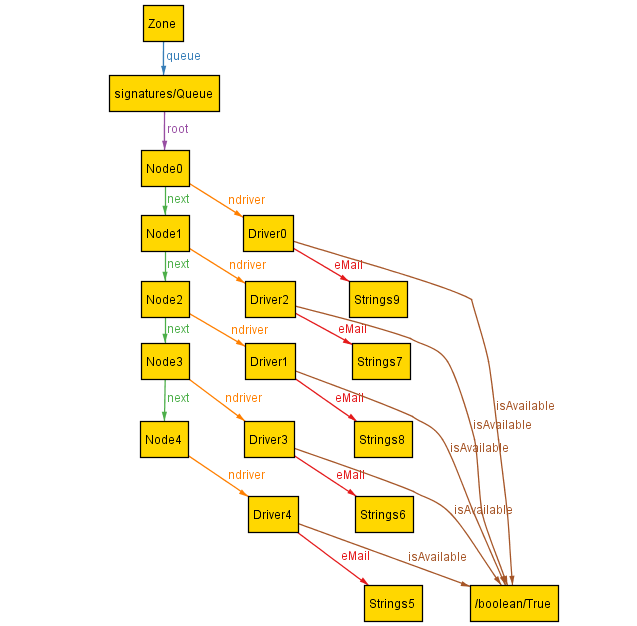
\includegraphics[width=\worldsWidth]{Alloy-AllAvailable}
\centering
\caption[Alloy World with all the Taxi Drivers Available]{This alloy world represents a particular situation in which all the Taxi Drivers are available. This is useful to see how the queue is implemented. Here is not present any Reservation}
\label{fig:alloyworldallavailable}
\end{figure}

\begin{figure}[H]
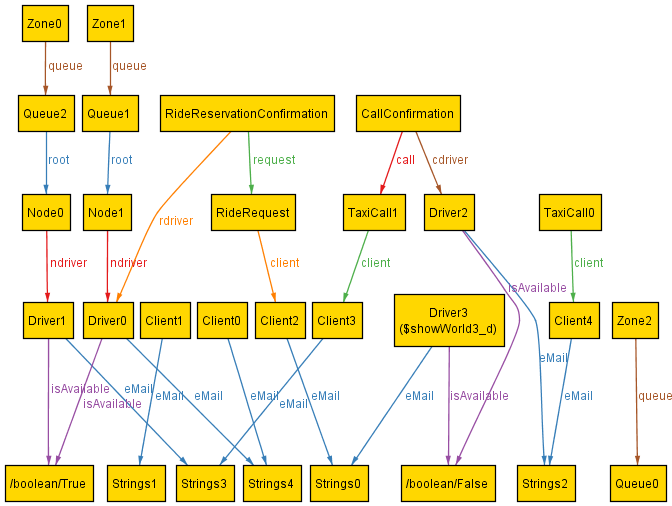
\includegraphics[width=\worldsWidth]{Alloy-FreeDriver}
\centering
\caption[Alloy World with a Taxi Driver in a rest]{This alloy world represents a situation in which you can show all the possible states of a Taxi Driver: Driver 0 is available but has a reservation accepted, Driver 1 is available, Driver 2 is busy in a Call and Driver 3 is at rest.
}
\label{fig:alloyworldfreedriver}
\end{figure}

\begin{figure}[H]
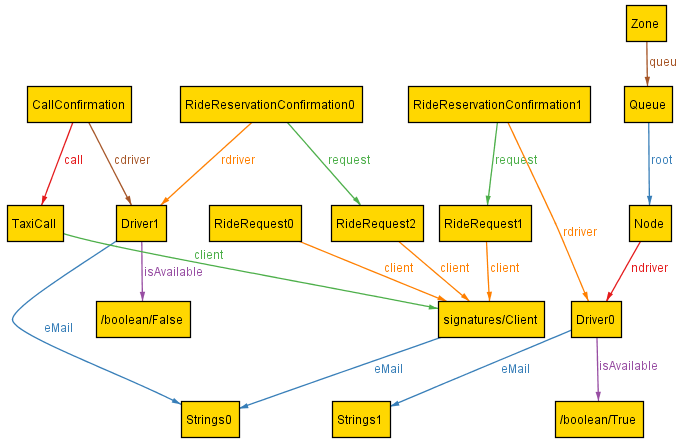
\includegraphics[width=\worldsWidth]{Alloy-RideReservation}
\centering
\caption[Alloy World with some Ride Reservations]{This alloy world was made to show a situation with some Ride Reservations mixed with Calls}
\label{fig:alloyworldridereservation}
\end{figure}

\subsection{Software and Tools used}

\begin{description}
\item[ShareLatex:] This web application was used to redact this document in a collaborative way. 
\newline (\url{https://it.sharelatex.com/})
\item[NinjaMock:] This online service was useful for design the mockups present in this document.
\newline (\url{https://ninjamock.com/})
\item[Creately:] This web service helped us to create Use Case Diagrams.
\newline (\url{https://creately.com})
\item[Astah Professional:] This desktop application was used to create all the others UML Diagrams.
\newline (\url{http://astah.net/})
\item[Signavio Academic:] This web application was used to create the BPMN diagrams
\newline (\url{http://academic.signavio.com})
\item[Alloy Analizer:] This tool was used to prove the consistency of our model.
\newline (\url{http://alloy.mit.edu/alloy/})
\end{description}

\subsection{Hours of Work}
We spent approximately the following amount of hours to redact this document:
\begin{description}
\item[Riva Luca:] 35
\item[Strada Jacopo:] 35
\end{description}

\end{document}